\section{Exploratory Data Analysis and Results}\label{sec:eda}

Age, smoking history and COPD separate people with and without lung cancer far more than any regional factor does. Fourteen of our eighteen tests stay significant after correction, but the effect sizes remind us that with 150,000 rows ``significant'' and ``important'' are not the same thing. For every test we followed the same checklist: state H$_0$, check the assumptions, run the test, report an effect size, and say what it means in plain words. Unless stated otherwise, $p$-values in the text are raw (before correction); Holm-adjusted values are always labelled ``Holm $p$''.

\subsection{Descriptive statistics and univariate analysis}\label{sec:univariate}

\textbf{The big picture.} \nAdults adults; mean age 52.8 years (SD 18.4), median 54 (IQR 37--68); 54.3\% women; \nCases lung-cancer cases (\sampleRate\% of the sample, 0.31\% once we apply the NHIS survey weights). The gap between the two rates is not a bug: the sample is older than the US population, so we use weighted rates whenever we talk about the population. The composition of the sample by every variable is described in Section~\ref{sec:profile}.

\begin{itemize}
  \item \textbf{Age is not normal.} It is flat with two humps (negative excess kurtosis, $-1.08$; Table~\ref{tab:numeric}) and a spike at the top-code. Both normality tests reject normality: Shapiro--Wilk on a random sample of 5,000 ages, $p = 5.7 \times 10^{-33}$, and D'Agostino's $K^2$ on all adults, $p < 10^{-300}$. The Q-Q plot confirms it visually (Fig.~\ref{fig:numeric}). We therefore use rank-based methods (Mann--Whitney, Spearman) for age, as the course recommends when normality fails (Chapter~4).
  \item \textbf{Comorbidity count is right-skewed} (skewness 1.29): half of adults have none of the five conditions, 31.7\% have one, and only 5.0\% have three or more.
  \item \textbf{No transformation is needed.} The only skewed column is a small count from 0 to 5, not a long-tailed amount such as income, so a log transform would not help; the regional columns are roughly symmetric.
\end{itemize}

\begin{table}[htbp]
\centering\small
\caption{Centre, spread and shape of the numeric columns (all \nAdults adults with the value known, unweighted).}\label{tab:numeric}
\begin{tabular}{lrrrrrrrr}
\toprule
Column & Mean & Median & SD & IQR & Min & Max & Skewness & \makecell[b]{Excess\\{}kurtosis} \\
\midrule
age (years) & 52.8 & 54.0 & 18.4 & 31.0 & 18.0 & 85.0 & $-$0.05 & $-$1.08 \\
comorbidity\_count & 0.73 & 0.00 & 0.91 & 1.00 & 0.00 & 5.00 & 1.29 & 1.54 \\
pm25\_mean (\textmu g/m$^3$) & 7.29 & 7.27 & 0.76 & 0.99 & 5.80 & 8.73 & $-$0.06 & $-$0.71 \\
smoking\_rate (\%) & 14.47 & 14.49 & 2.08 & 3.00 & 10.22 & 18.01 & $-$0.00 & $-$0.83 \\
lung\_cancer\_incidence (/100k) & 67.4 & 71.0 & 12.5 & 26.0 & 44.7 & 82.2 & $-$0.87 & $-$0.81 \\
\bottomrule
\end{tabular}

\end{table}

\begin{figure}[htbp]
\centering
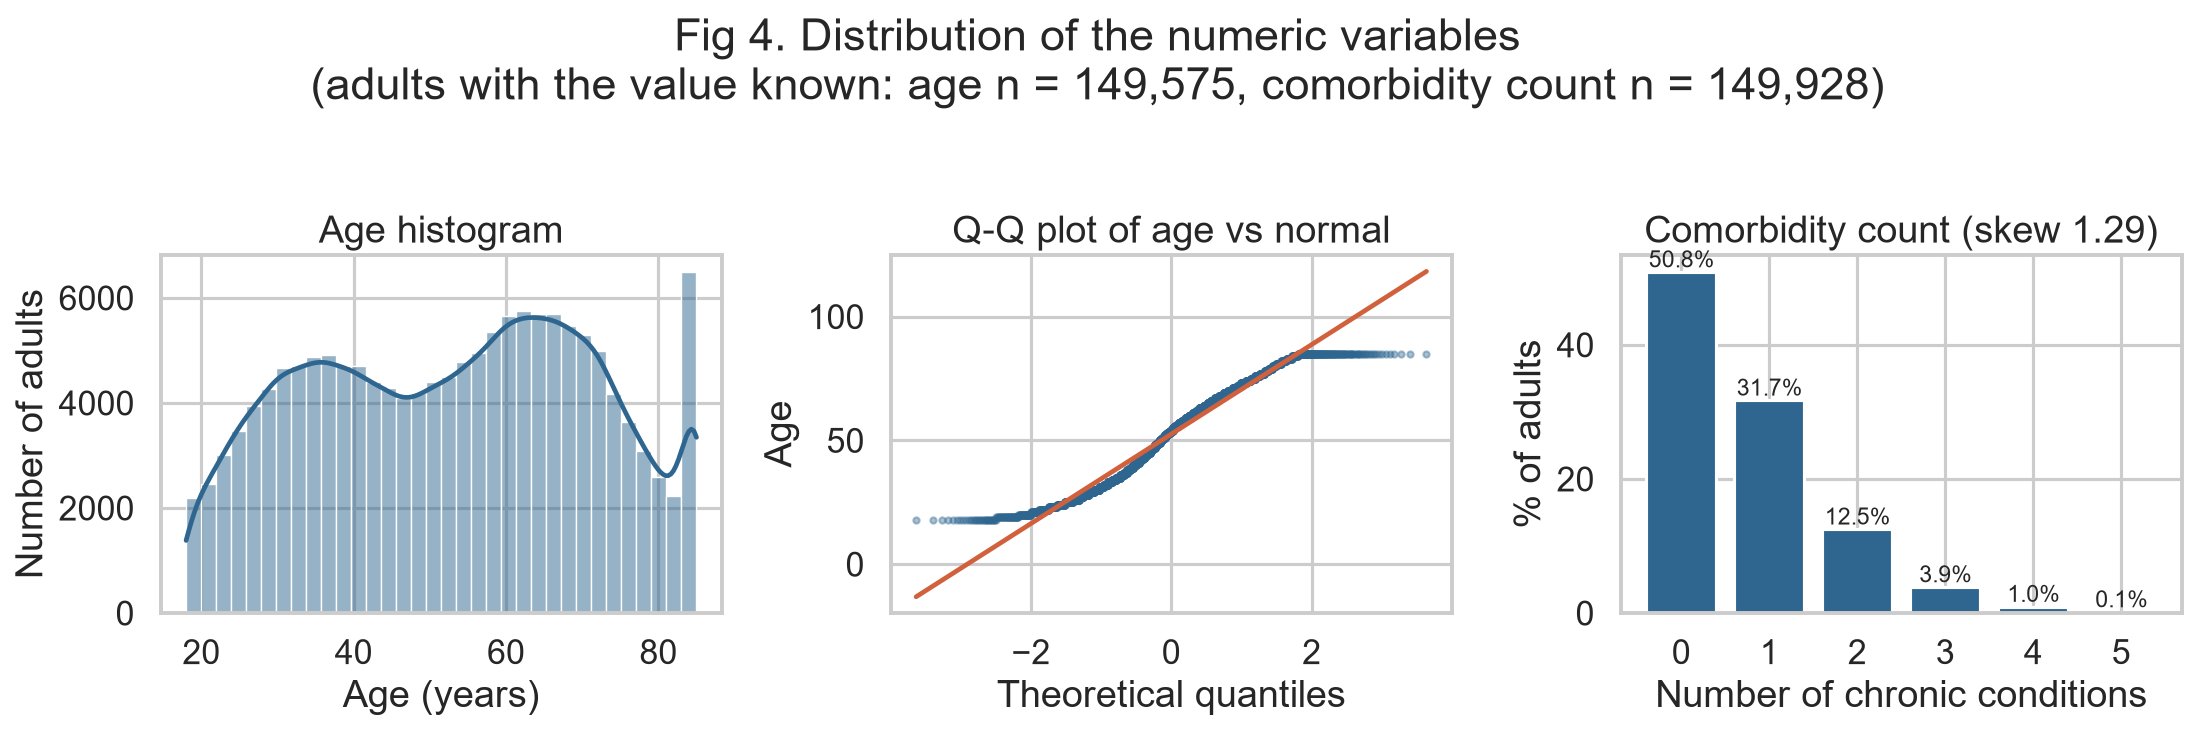
\includegraphics[width=\textwidth]{fig04_numeric_distributions}
\caption{Numeric variables. Left: age histogram (two humps, and a pile-up at 85 = ``85 or older''). Centre: Q-Q plot of age against a normal distribution (the S-shape of a flat distribution). Right: comorbidity count (right-skewed).}\label{fig:numeric}
\end{figure}

\begin{figure}[htbp]
\centering
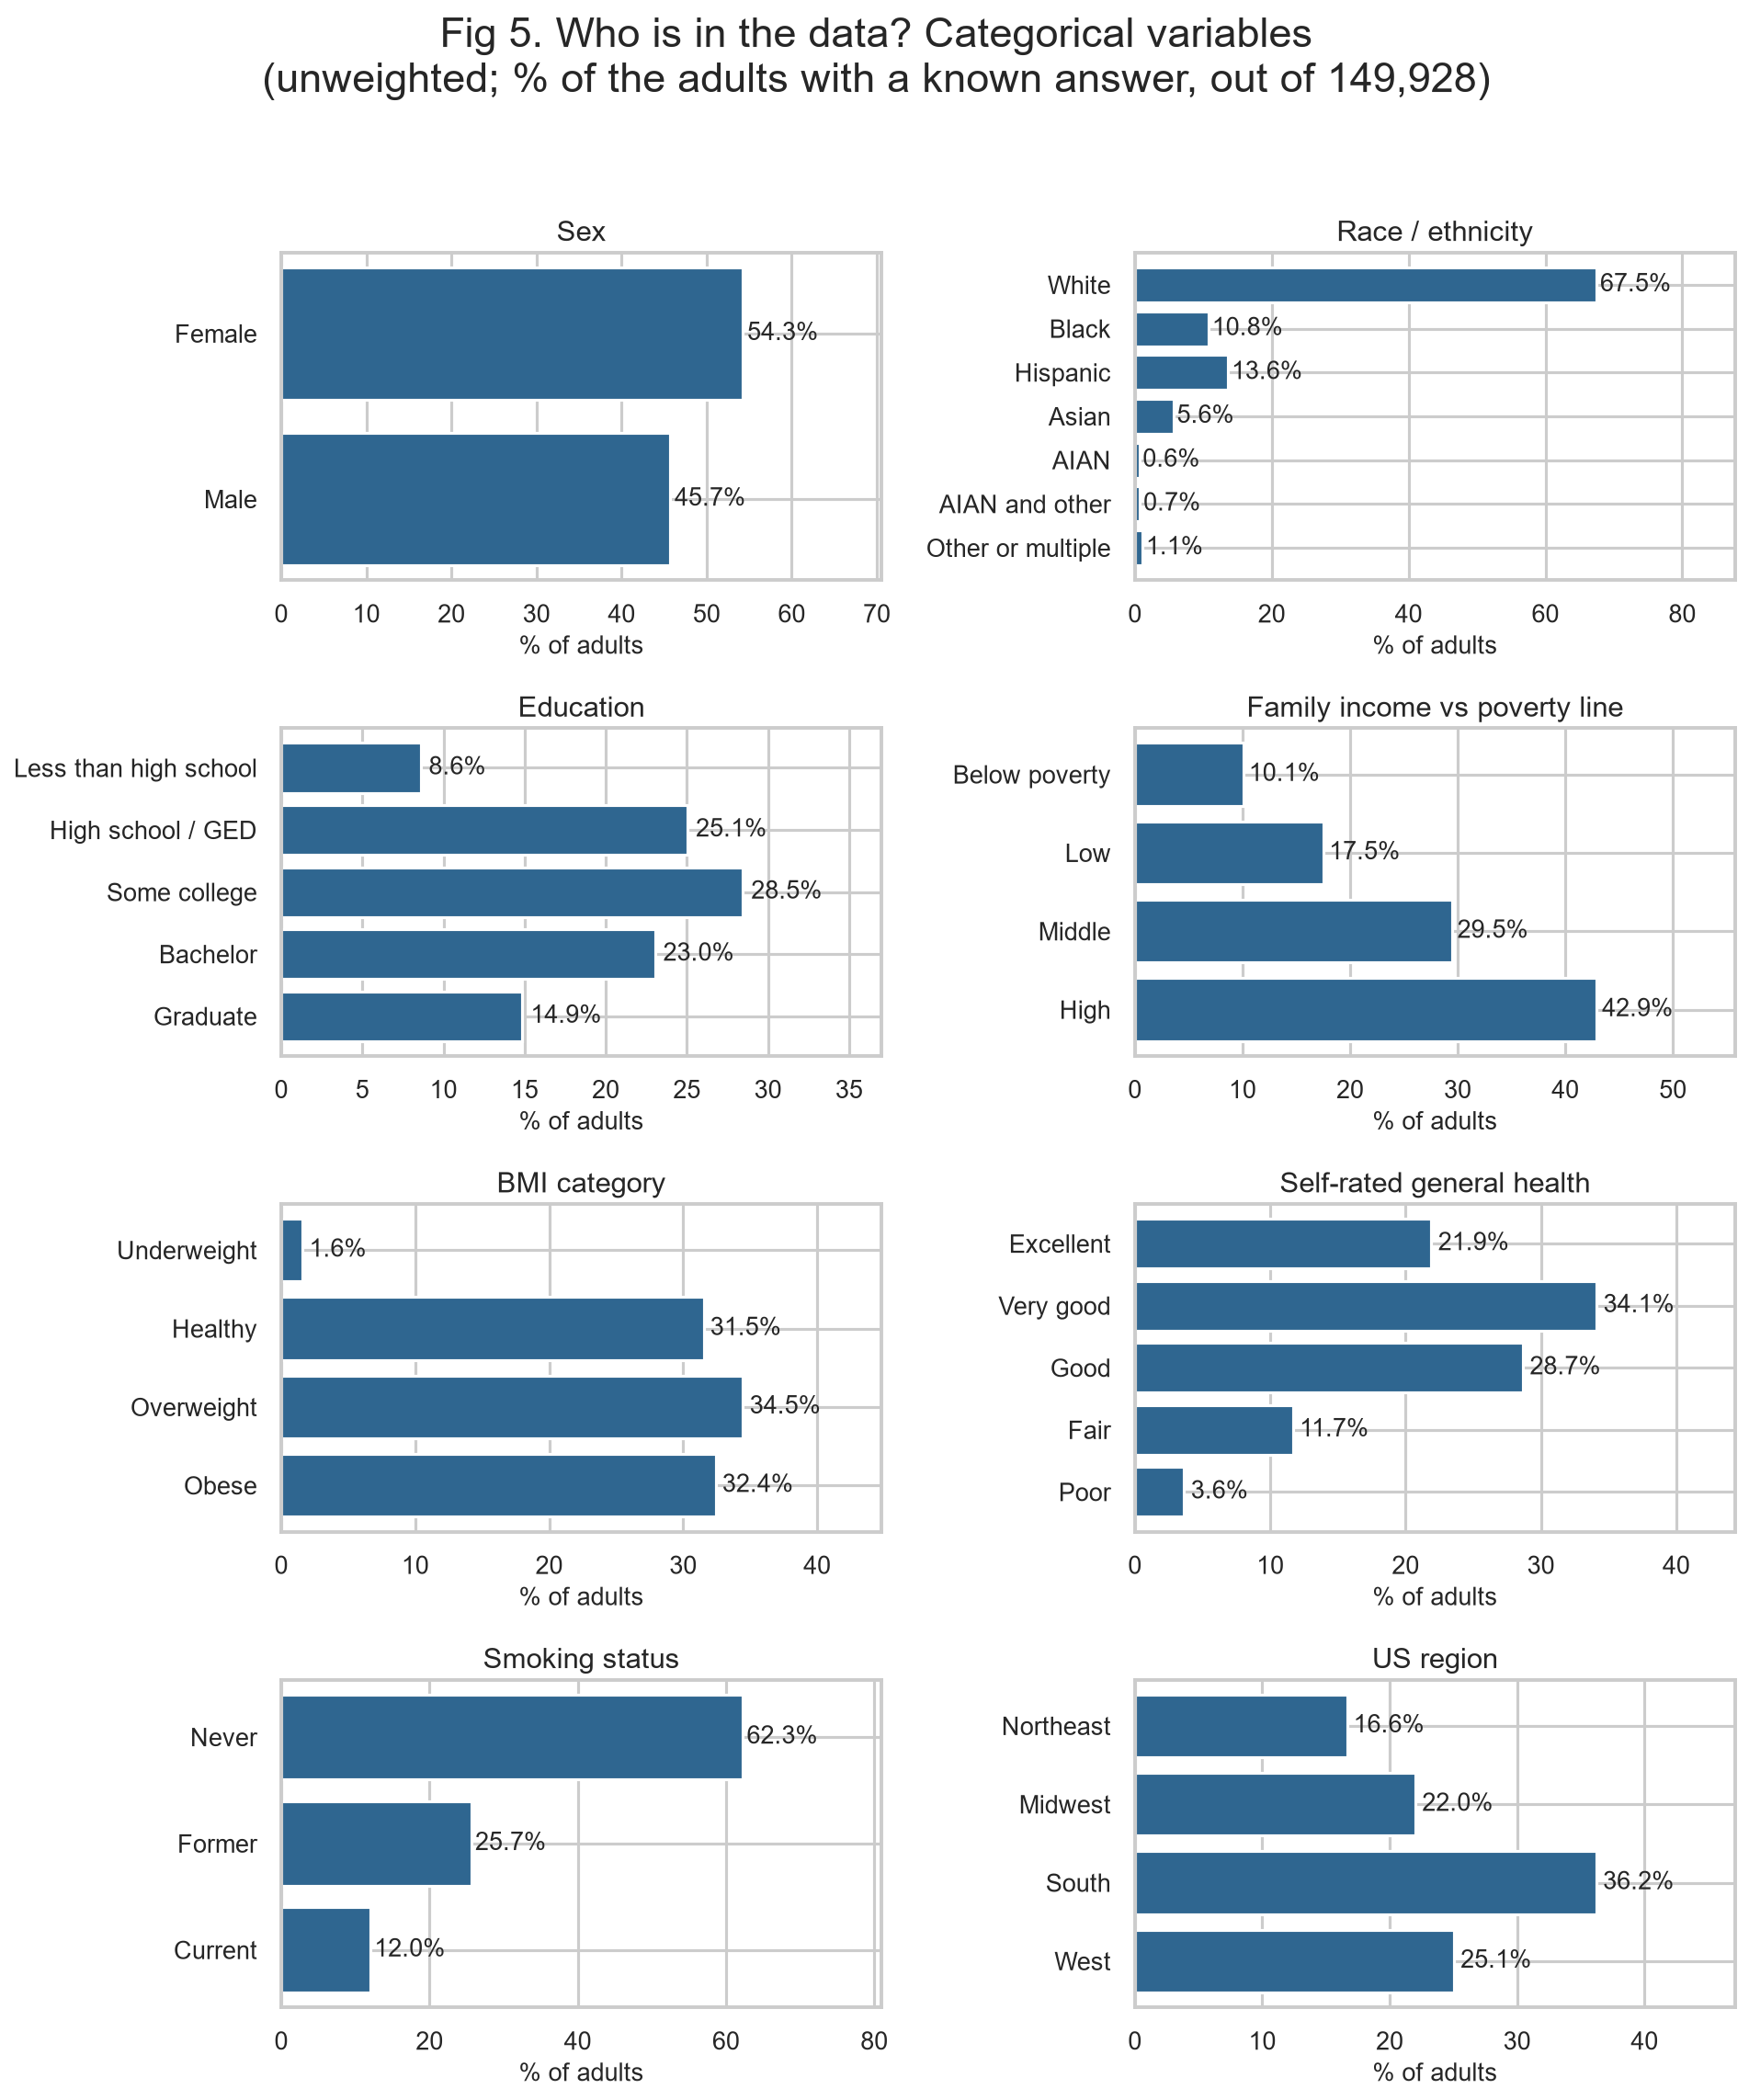
\includegraphics[width=0.85\textwidth]{fig05_categorical_distributions}
\caption{Distribution of the categorical variables (unweighted shares of adults with a known answer). Counts, cases and rates for every category are in Tables~\ref{tab:prof-demo}--\ref{tab:prof-conditions}.}\label{fig:categorical}
\end{figure}

\subsection{RQ1 -- Smoking}\label{sec:rq1}

\begin{table}[htbp]
\centering\small
\caption{Lung-cancer rate by smoking status (absolute risk) and risk ratio against never-smokers (adults with known smoking status).}\label{tab:rate-smoking}
\begin{tabular}{lrrrrr}
\toprule
Smoking status & Adults & Cases & \makecell[b]{Sample\\{}rate} & \makecell[b]{Weighted\\{}(population) rate} & \makecell[b]{Risk ratio\\{}(weighted)} \\
\midrule
Never & 90,937 & 107 & 0.12\% & 0.08\% & 1 (reference) \\
Former & 37,452 & 367 & 0.98\% & 0.81\% & 10.0 \\
Current & 17,586 & 127 & 0.72\% & 0.60\% & 7.4 \\
\bottomrule
\end{tabular}

\end{table}

\begin{itemize}
  \item \textbf{Hypotheses.} H$_0$: smoking status and lung cancer are independent; H$_1$: they are associated.
  \item \textbf{Test and assumption.} Both variables are categorical (a $3 \times 2$ table), so we use Pearson's $\chi^2$ test of independence. Its assumption holds: the smallest expected count is 72.4, far above 5.
  \item \textbf{Result.} $\chi^2(2) = 528.0$, $p = 2.2 \times 10^{-115}$ (Holm $p = 3.1 \times 10^{-114}$), Cram\'er's $V = 0.060$ -- small by Cohen's conventions~\cite{cohen}.
  \item \textbf{Effect size.} Ever-smokers vs never-smokers: odds ratio \orSmokingExact (95\% CI 6.22--9.44). In absolute terms, about 8 in 10,000 never-smokers have a lung-cancer history in the population, against about 81 in 10,000 former and 60 in 10,000 current smokers (Table~\ref{tab:rate-smoking}, Fig.~\ref{fig:smoking}).
  \item \textbf{How we read it.} The tiny $p$-value mostly reflects our sample size, and $V$ looks small because 99.6\% of every group is cancer-free -- $V$ is bounded by the rarity of the outcome. The odds ratio is the meaningful effect size for a rare outcome: ever-smokers have about \orSmoking times the odds of a lung-cancer history.
  \item \textbf{Why former smokers look worse than current ones (0.81\% vs 0.60\%).} At first this looked like a bug, but it is not one. NHIS records smoking now, and many people quit after their diagnosis, which moves them into the ``former'' group (reverse causation). Former smokers are also older (median age 63 vs 52 for current smokers), which is why we look at age next.
\end{itemize}

\begin{figure}[htbp]
\centering
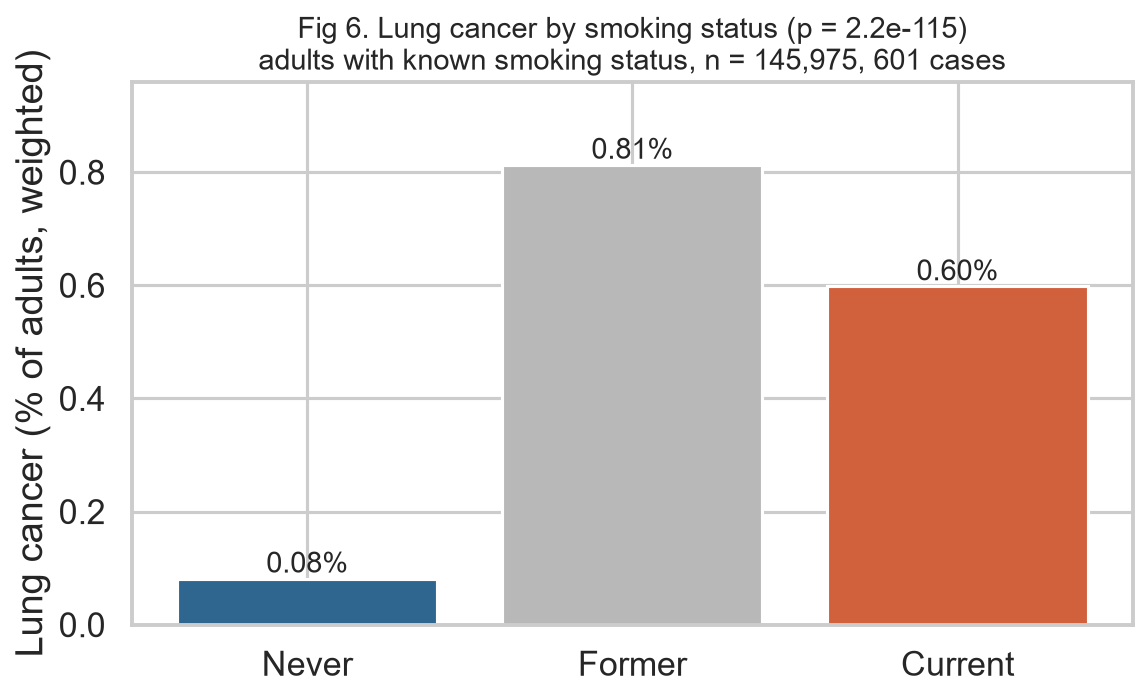
\includegraphics[width=0.6\textwidth]{fig06_smoking_vs_lung_cancer}
\caption{Weighted share of adults with a lung-cancer history, by smoking status (the $p$-value in the title is the raw $\chi^2$ $p$-value).}\label{fig:smoking}
\end{figure}

\subsection{RQ2a -- Age, and how it interacts with smoking}\label{sec:age}

\begin{figure}[htbp]
\centering
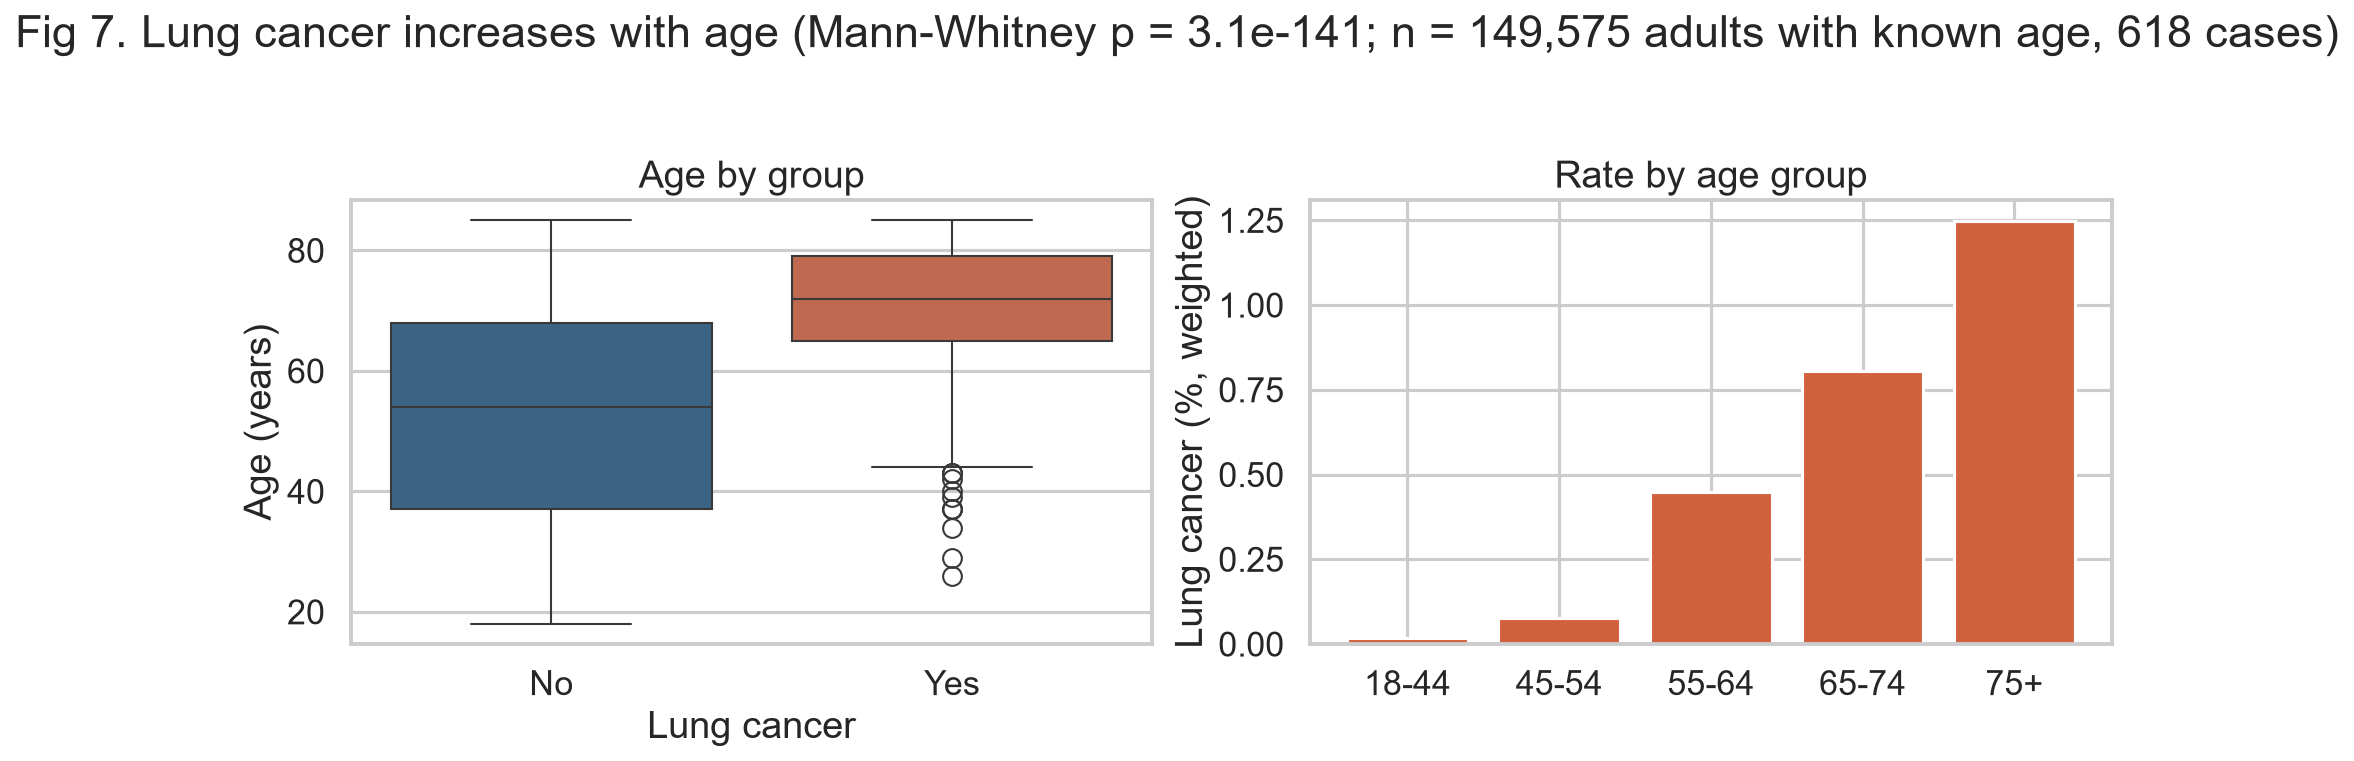
\includegraphics[width=\textwidth]{fig07_age_vs_lung_cancer}
\caption{Left: age distribution with and without lung cancer. Right: weighted lung-cancer rate by age group.}\label{fig:age}
\end{figure}

\begin{itemize}
  \item \textbf{Difference.} The median age is 72 with lung cancer vs 54 without, and the weighted rate rises steadily from the youngest to the oldest age group (Fig.~\ref{fig:age}).
  \item \textbf{Test choice.} H$_0$: both groups have the same age distribution. Age is not normal (\S\ref{sec:univariate}) and the groups are very unequal (618 vs 148,957 adults with a known age), so we use the Mann--Whitney $U$ test rather than a $t$-test.
  \item \textbf{Result.} $U = 73{,}126{,}291$, $p = 3.1 \times 10^{-141}$, rank-biserial $r = 0.59$ -- a large effect. In plain words: if we pick one adult with and one without a lung-cancer history at random, the one with lung cancer is older $(1 + 0.59)/2 \approx 79.5\%$ of the time.
  \item \textbf{Robustness.} With samples this large the $t$-test is also valid (central limit theorem), so we ran Welch's $t$-test as a check: $t = 44.9$, $p = 4.6 \times 10^{-199}$. Both tests agree, so the conclusion does not depend on the choice of test.
\end{itemize}

\begin{figure}[htbp]
\centering
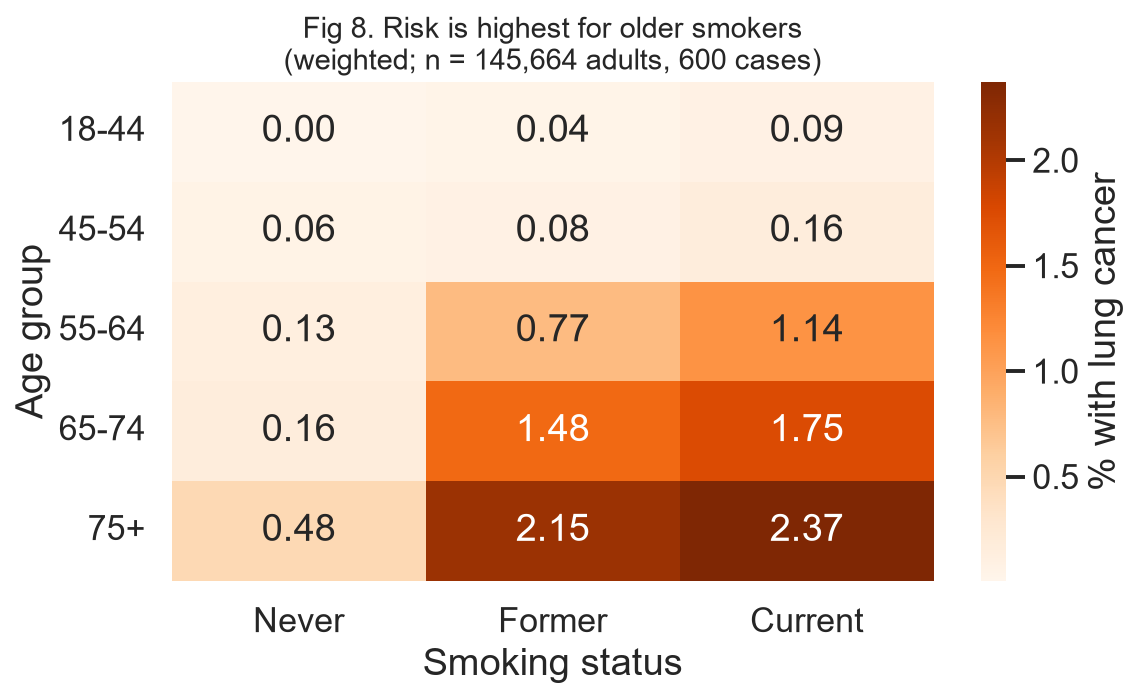
\includegraphics[width=0.6\textwidth]{fig08_age_x_smoking}
\caption{Weighted lung-cancer rate (\%) for each age group and smoking status. Cells for adults under 45 contain very few cases (3 never-smokers and 10 ever-smokers in total), so their rates are imprecise.}\label{fig:agesmoking}
\end{figure}

\begin{itemize}
  \item \textbf{Age and smoking act together.} Never-smokers stay below 0.5\% even at 75+. Ever-smokers go from under 0.1\% before 45 to 2.15\% (former) and 2.37\% (current) at 75+.
  \item \textbf{Smoking is not just age in disguise -- tested.} Because ever-smokers are older, part of the crude odds ratio could be age. We therefore compared ever- with never-smokers inside each age group and pooled the groups with the Cochran--Mantel--Haenszel (CMH) method (Table~\ref{tab:smoking-age}). The odds ratio falls from 7.6 to \orSmokingMH (95\% CI 4.7--7.1) once age group is held fixed, and the CMH test rejects ``no association within age groups'' ($\chi^2 = 340.5$, $p = 5 \times 10^{-76}$). Part of the crude effect was therefore age, but a strong smoking association remains. The Breslow--Day test ($p = 0.005$) shows the size of the effect differs between age groups: it is about 8 from 55 to 74, 4.4 at 75+, and not significant at 45--54 (only 21 cases), so the pooled \orSmokingMH is an average.
  \item This combination of age and smoking is exactly the logic of the USPSTF screening rule, which combines age 50--80 with smoking history -- and the reason we built the \file{screening_age_smoker} feature (\S\ref{sec:created}, Table~\ref{tab:engineered}).
\end{itemize}

\begin{table}[htbp]
\centering\small
\caption{Smoking and lung cancer inside each age group (ever vs never smokers; adults with known smoking status and age). CMH $\chi^2 = 340.5$, $p = 5 \times 10^{-76}$; Breslow--Day $p = 0.005$. Source: \texttt{smoking\_by\_age\_group.csv}.}\label{tab:smoking-age}
\begin{tabular}{lrrrr}
\toprule
Age group & Adults & \makecell[b]{Cases,\\{}ever-smokers} & \makecell[b]{Cases,\\{}never-smokers} & Odds ratio [95\% CI] \\
\midrule
18--44 & 53,022 & 10 & 3 & 7.7 [2.3, 25.9] \\
45--54 & 20,987 & 11 & 10 & 1.9 [0.8, 4.3] \\
55--64 & 26,358 & 96 & 15 & 8.2 [4.8, 14.0] \\
65--74 & 25,842 & 187 & 27 & 7.9 [5.3, 11.7] \\
75+ & 19,455 & 189 & 52 & 4.4 [3.2, 5.9] \\
\midrule
Crude (age ignored) & 145,664 &  &  & 7.6 [6.2, 9.4] \\
Mantel--Haenszel (adjusted for age group) & 145,664 &  &  & 5.8 [4.7, 7.1] \\
\bottomrule
\end{tabular}

\end{table}

\subsection{RQ2b -- Chronic conditions}\label{sec:conditions}

\begin{figure}[htbp]
\centering
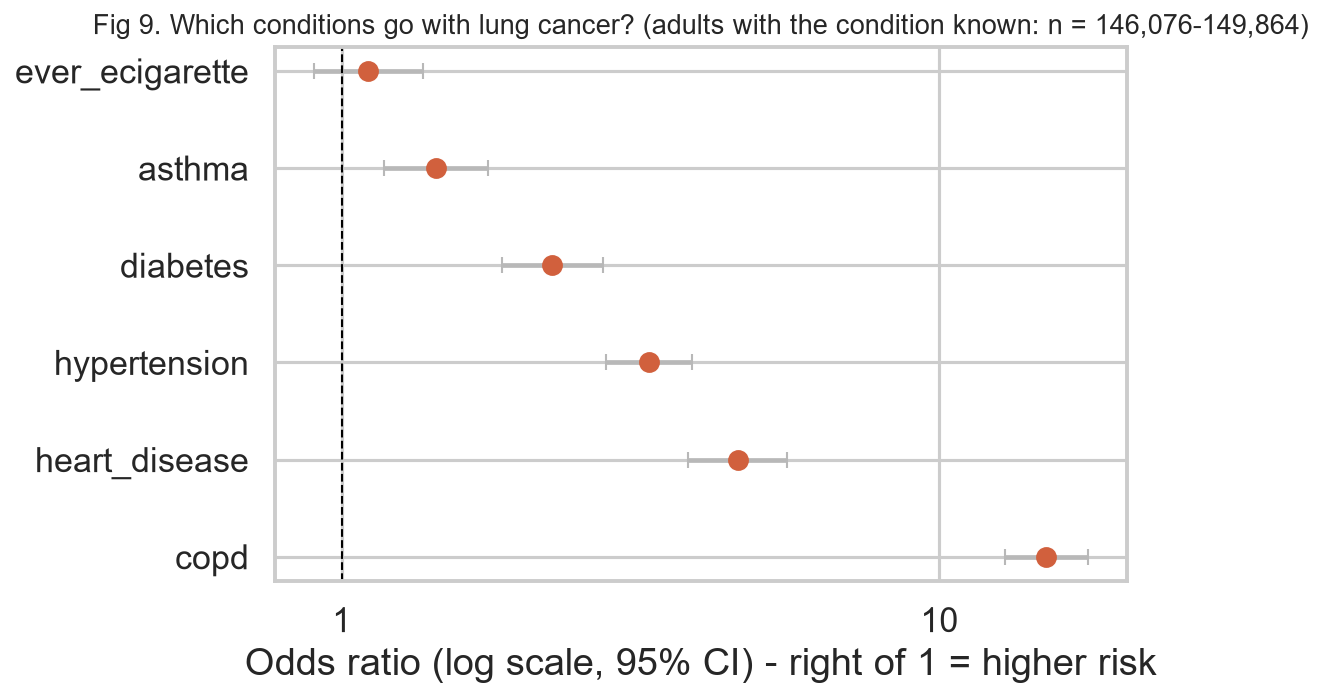
\includegraphics[width=0.65\textwidth]{fig09_odds_ratios_conditions}
\caption{Odds ratio of a lung-cancer history for each condition, with 95\% confidence intervals (log scale). Right of 1 means higher odds.}\label{fig:conditions}
\end{figure}

\begin{table}[htbp]
\centering\small
\caption{Chronic conditions and e-cigarette use vs lung cancer ($\chi^2$ tests; all expected counts $\geq 5$).}\label{tab:conditions}
\begin{tabular}{lrrrrr}
\toprule
Condition & \makecell[b]{Rate\\{}if yes} & \makecell[b]{Rate\\{}if no} & \makecell[b]{Odds ratio\\{}[95\% CI]} & Cram\'er's $V$ & Holm $p$ \\
\midrule
COPD & 3.41\% & 0.23\% & 15.1 [12.9, 17.7] & 0.114 & $<10^{-300}$ \\
Heart disease & 1.53\% & 0.34\% & 4.6 [3.8, 5.6] & 0.045 & $7.3\times10^{-65}$ \\
Hypertension & 0.74\% & 0.23\% & 3.3 [2.8, 3.9] & 0.038 & $1.5\times10^{-48}$ \\
Diabetes & 0.82\% & 0.36\% & 2.3 [1.9, 2.7] & 0.022 & $6.7\times10^{-16}$ \\
Asthma & 0.56\% & 0.39\% & 1.4 [1.2, 1.8] & 0.009 & $2.9\times10^{-3}$ \\
E-cigarette (ever) & 0.45\% & 0.41\% & 1.1 [0.9, 1.4] & 0.002 & 1.00 \\
\bottomrule
\end{tabular}

\end{table}

\begin{itemize}
  \item \textbf{COPD is the strongest signal in the whole project.} It shares smoking as a cause and is also a known risk factor on its own -- which is why we test it against smoking (and age) in \S\ref{sec:copd}.
  \item \textbf{Heart disease, hypertension and diabetes} are partly proxies for age; these odds ratios (Fig.~\ref{fig:conditions}) are not age-adjusted, so we do not over-read them.
  \item \textbf{Asthma} survives correction, but its effect is negligible ($V = 0.009$): a clear example of significant without being important.
  \item \textbf{E-cigarette use shows nothing} (raw $p = 0.39$, Holm $p = 1.00$). That makes sense: e-cigarettes are recent, users are mostly young (mean age 41 vs 55 for non-users, Table~\ref{tab:prof-smoking}), and lung cancer takes decades to develop. Section~\ref{sec:notshow} reports what this null result can and cannot rule out.
\end{itemize}

\subsection{RQ2b -- Is the COPD link only due to smoking?}\label{sec:copd}

Smokers develop COPD more often and lung cancer more often, so smoking alone could create a COPD--lung-cancer association -- a classic confounder. To separate the two, we compared adults with and without COPD within each smoking group (Fig.~\ref{fig:copd}, Table~\ref{tab:copd-smoking}), then pooled the three groups with the Cochran--Mantel--Haenszel (CMH) test~\cite{mantel}, which tests H$_0$: ``no COPD--lung-cancer association once smoking status is held fixed''.

\begin{figure}[htbp]
\centering
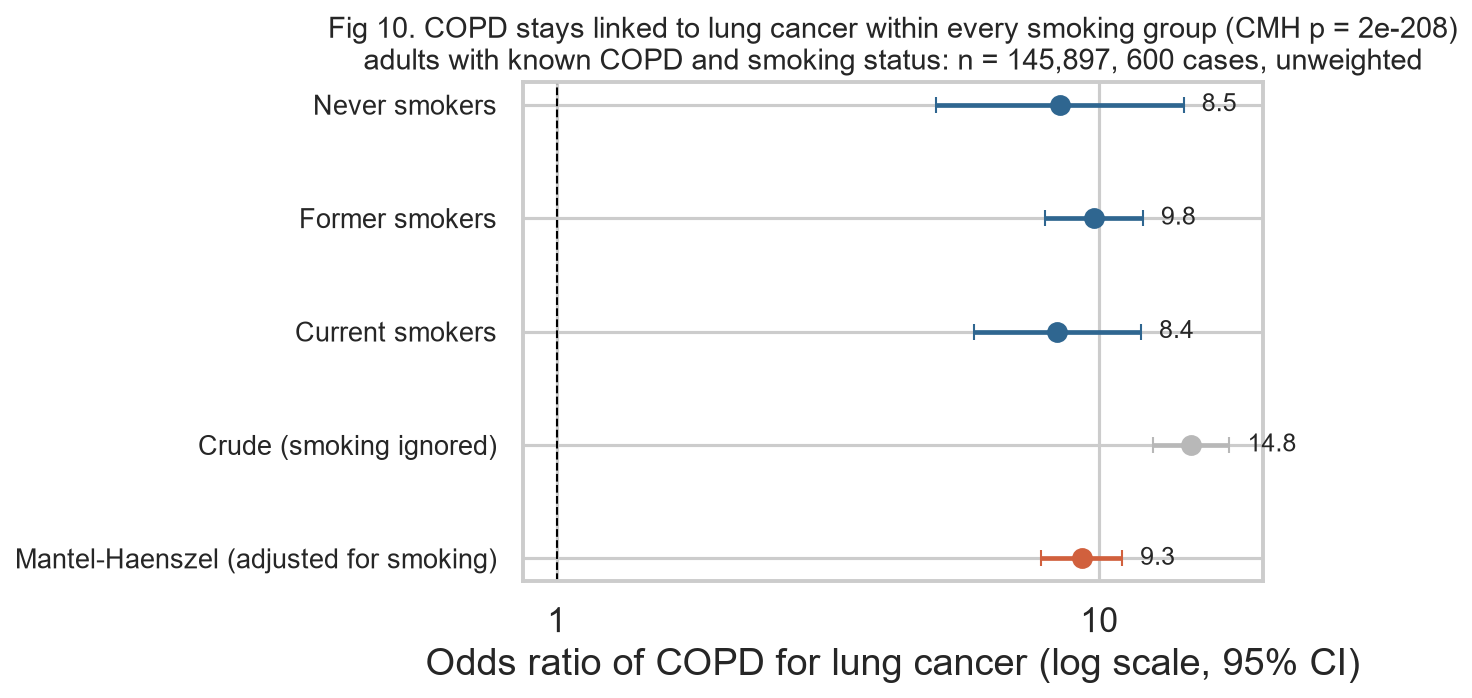
\includegraphics[width=0.75\textwidth]{fig10_copd_stratified_by_smoking}
\caption{Odds ratio of COPD for lung cancer within each smoking group, ignoring smoking (crude) and adjusted for smoking (Mantel--Haenszel), with 95\% confidence intervals (log scale).}\label{fig:copd}
\end{figure}

\begin{table}[htbp]
\centering\small
\caption{COPD and lung cancer, stratified by smoking status (adults with known COPD and smoking status).}\label{tab:copd-smoking}
\begin{tabular}{lrrr}
\toprule
Group & Adults & Cases & Odds ratio [95\% CI] \\
\midrule
Never smokers & 90,901 & 107 & 8.5 [5.0, 14.3] \\
Former smokers & 37,424 & 366 & 9.8 [7.9, 12.0] \\
Current smokers & 17,572 & 127 & 8.4 [5.9, 11.9] \\
\midrule
Crude (smoking ignored) & 145,897 & 600 & 14.8 [12.6, 17.4] \\
Mantel--Haenszel (adjusted for smoking) & 145,897 & 600 & 9.3 [7.8, 11.0] \\
\bottomrule
\end{tabular}

\end{table}

\begin{itemize}
  \item \textbf{CMH test:} $\chi^2 = 949.7$, $p = 1.5 \times 10^{-208}$ (Holm $p = 2.4 \times 10^{-207}$) -- the association survives adjustment for smoking.
  \item \textbf{Breslow--Day test} of equal odds ratios across the three groups: $p = 0.69$, so the effect is consistent across groups and pooling them is justified.
  \item \textbf{How we read it.} The crude odds ratio of these 145,897 adults is \orCOPDcrude (slightly below the \orCOPD of Table~\ref{tab:conditions}, which uses everyone with a known COPD answer); it falls to \orCOPDsmoking once smoking is held fixed, so part of the crude association was due to smoking. But COPD remains strongly associated with lung cancer in never, former and current smokers alike -- even never-smokers with COPD have 8.5 times the odds.
  \item \textbf{Age as a second confounder.} Adults with COPD are much older (mean age 65.4 vs 52.0). On the 145,587 adults whose age is also known (599 cases), the crude odds ratio is 14.7 and the smoking-adjusted one 9.2 -- the same picture as above -- and stratifying by smoking status and age group together (15 strata; Table~\ref{tab:copd-adjusted}) lowers it further, to \orCOPDsmokingAge (95\% CI 4.8--6.8), still highly significant ($\chi^2 = 501.9$, $p = 3.7 \times 10^{-111}$). COPD is therefore strongly associated with lung cancer beyond what smoking and age explain -- still an association, not a cause.
\end{itemize}

\begin{table}[htbp]
\centering\small
\caption{COPD odds ratio under increasing adjustment (the 145,587 adults with known COPD, smoking status and age; 599 cases). Source: \texttt{copd\_adjusted.csv}.}\label{tab:copd-adjusted}
\begin{tabular}{lr}
\toprule
Adjusted for & Odds ratio [95\% CI] \\
\midrule
None (crude) & 14.7 [12.5, 17.3] \\
Smoking status (3 strata) & 9.2 [7.8, 11.0] \\
Smoking status $\times$ age group (15 strata) & 5.7 [4.8, 6.8] \\
\bottomrule
\end{tabular}

\end{table}

\subsection{RQ2c -- Socio-demographic and health factors}\label{sec:sociodemo}

\begin{figure}[htbp]
\centering
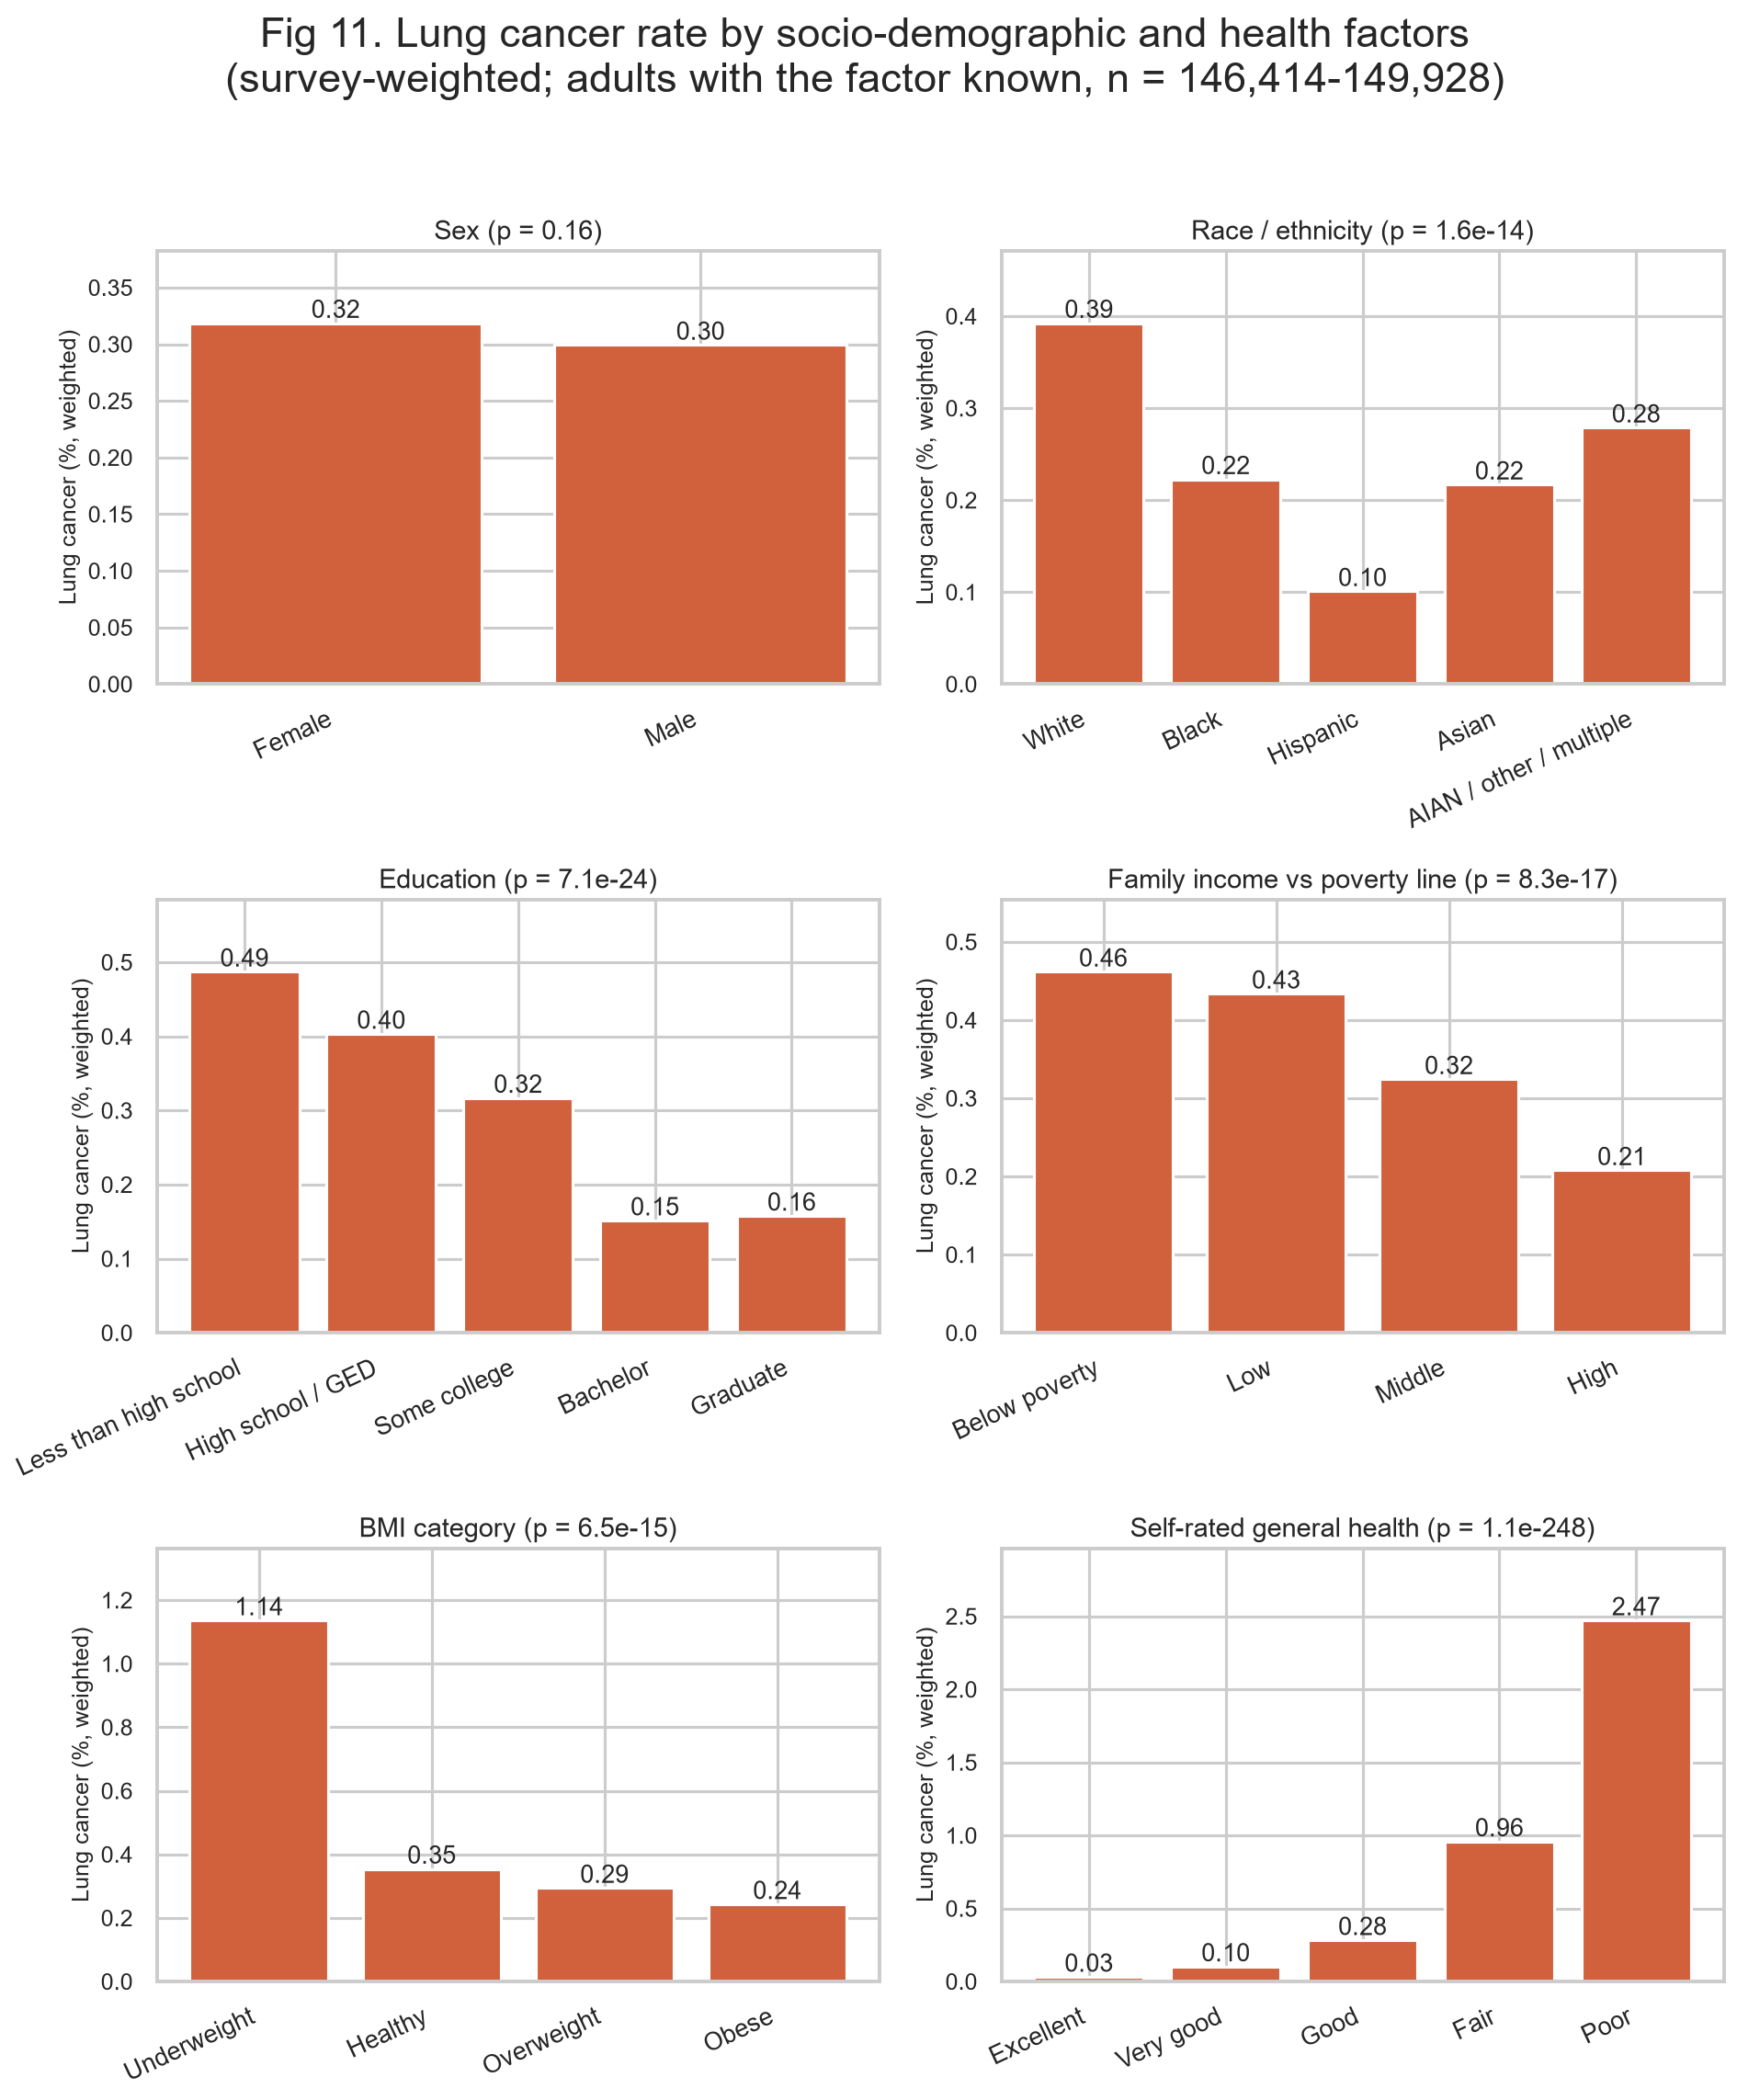
\includegraphics[width=0.85\textwidth]{fig11_demographics_vs_lung_cancer}
\caption{Weighted lung-cancer rate (\%) by sex, race/ethnicity, education, income, BMI category and self-rated general health, with the raw $\chi^2$ $p$-value of each test in the panel titles (Holm-adjusted values in Table~\ref{tab:demographics}).}\label{fig:demographics}
\end{figure}

\begin{table}[htbp]
\centering\small
\caption{Socio-demographic and health factors vs lung cancer ($\chi^2$ tests of independence). The three smallest race groups (AIAN, AIAN and other, Other or multiple; 2.5\% of adults) were merged for the test, because their expected case counts fell below 5 (smallest 4.0), which makes the $\chi^2$ approximation unreliable. After merging, the smallest expected count is 15.5. The model-ready file keeps all seven groups as categories (White is the reference category).}\label{tab:demographics}
\begin{tabularx}{\textwidth}{l >{\raggedright\arraybackslash}X r r r}
\toprule
Factor & Weighted rate: highest $\rightarrow$ lowest group & $\chi^2$ (df) & Holm $p$ & Cram\'er's $V$ \\
\midrule
Sex & Female 0.32\% $\rightarrow$ Male 0.30\% & 2.0 (1) & 0.62 & 0.004 \\
Race / ethnicity & White 0.39\% $\rightarrow$ Hispanic 0.10\% & 70.7 (4) & $1.1\times10^{-13}$ & 0.022 \\
Education & Less than high school 0.49\% $\rightarrow$ Bachelor 0.15\% & 114.7 (4) & $7.8\times10^{-23}$ & 0.028 \\
Income vs poverty line & Below poverty 0.46\% $\rightarrow$ High 0.21\% & 78.0 (3) & $7.5\times10^{-16}$ & 0.023 \\
BMI category & Underweight 1.14\% $\rightarrow$ Obese 0.24\% & 69.2 (3) & $5.2\times10^{-14}$ & 0.022 \\
Self-rated health & Poor 2.47\% $\rightarrow$ Excellent 0.03\% & 1,154.7 (4) & $1.8\times10^{-247}$ & 0.088 \\
\bottomrule
\end{tabularx}

\end{table}

\begin{itemize}
  \item \textbf{Sex} is not associated with lung cancer here (raw $p = 0.16$, Holm $p = 0.62$; Table~\ref{tab:demographics}).
  \item \textbf{A social gradient.} Less education and lower income go with higher rates (Fig.~\ref{fig:demographics}). Smoking follows the same gradient -- 46\% of adults without a high-school diploma have ever smoked, against 28\% of bachelor's graduates, and 44\% below the poverty line against 33\% in the high-income group -- so part of this gradient is the smoking effect again.
  \item \textbf{Underweight and poor self-rated health have the highest rates.} This is most likely reverse causation: cancer and its treatment cause weight loss and poor health, not the other way round. These features describe people who are already sick, which matters for the modelling phase (\S\ref{sec:final}).
  \item \textbf{Race differences} may partly reflect differences in age and smoking between groups (Table~\ref{tab:group-profile}); they are not adjusted here. All Cram\'er's $V$ values are small, again because the outcome is rare. These tests treat education, income, BMI and health as nominal; a trend test that uses their order would be more powerful, which can only strengthen these already significant results.
\end{itemize}

\subsection{Correlations between variables}\label{sec:correlations}

\begin{figure}[htbp]
\centering
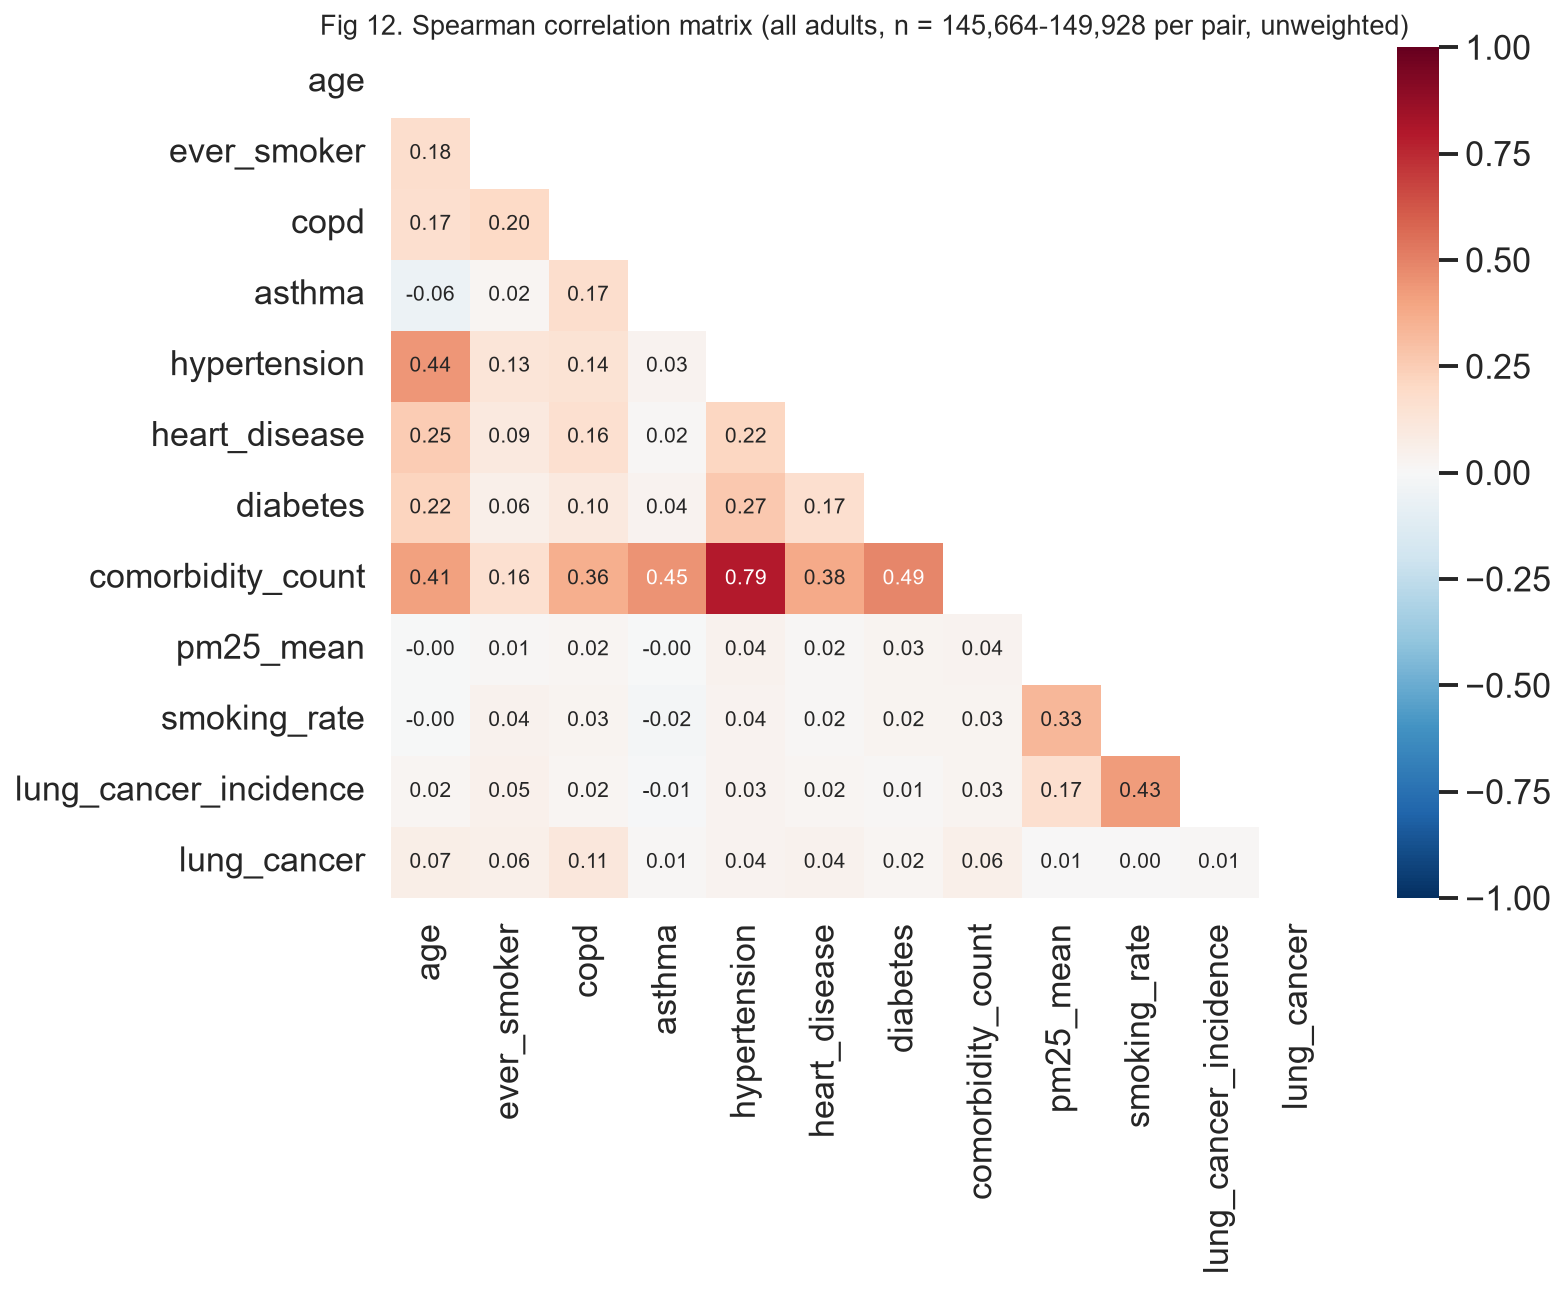
\includegraphics[width=0.7\textwidth]{fig12_correlation_heatmap}
\caption{Spearman correlation matrix of the numeric and binary variables (lower triangle; all adults, unweighted; each pair uses the adults with both values known, $n$ = 145,664--149,928).}\label{fig:corr}
\end{figure}

\begin{itemize}
  \item \textbf{Why Spearman.} Most columns are 0/1 or ordinal, and age is not normal; Spearman uses ranks and only assumes a monotonic relationship, whereas Pearson assumes linearity (Chapter~4).
  \item \textbf{The strongest pairs are expected.} Hypertension--comorbidity count (0.79), diabetes--comorbidity count (0.49) and asthma--comorbidity count (0.45) are high because the count is built from those columns. Age also goes with hypertension (0.44) and the comorbidity count (0.41), and the regional smoking rate with registry incidence (0.43).
\end{itemize}

\begin{figure}[p]
\centering
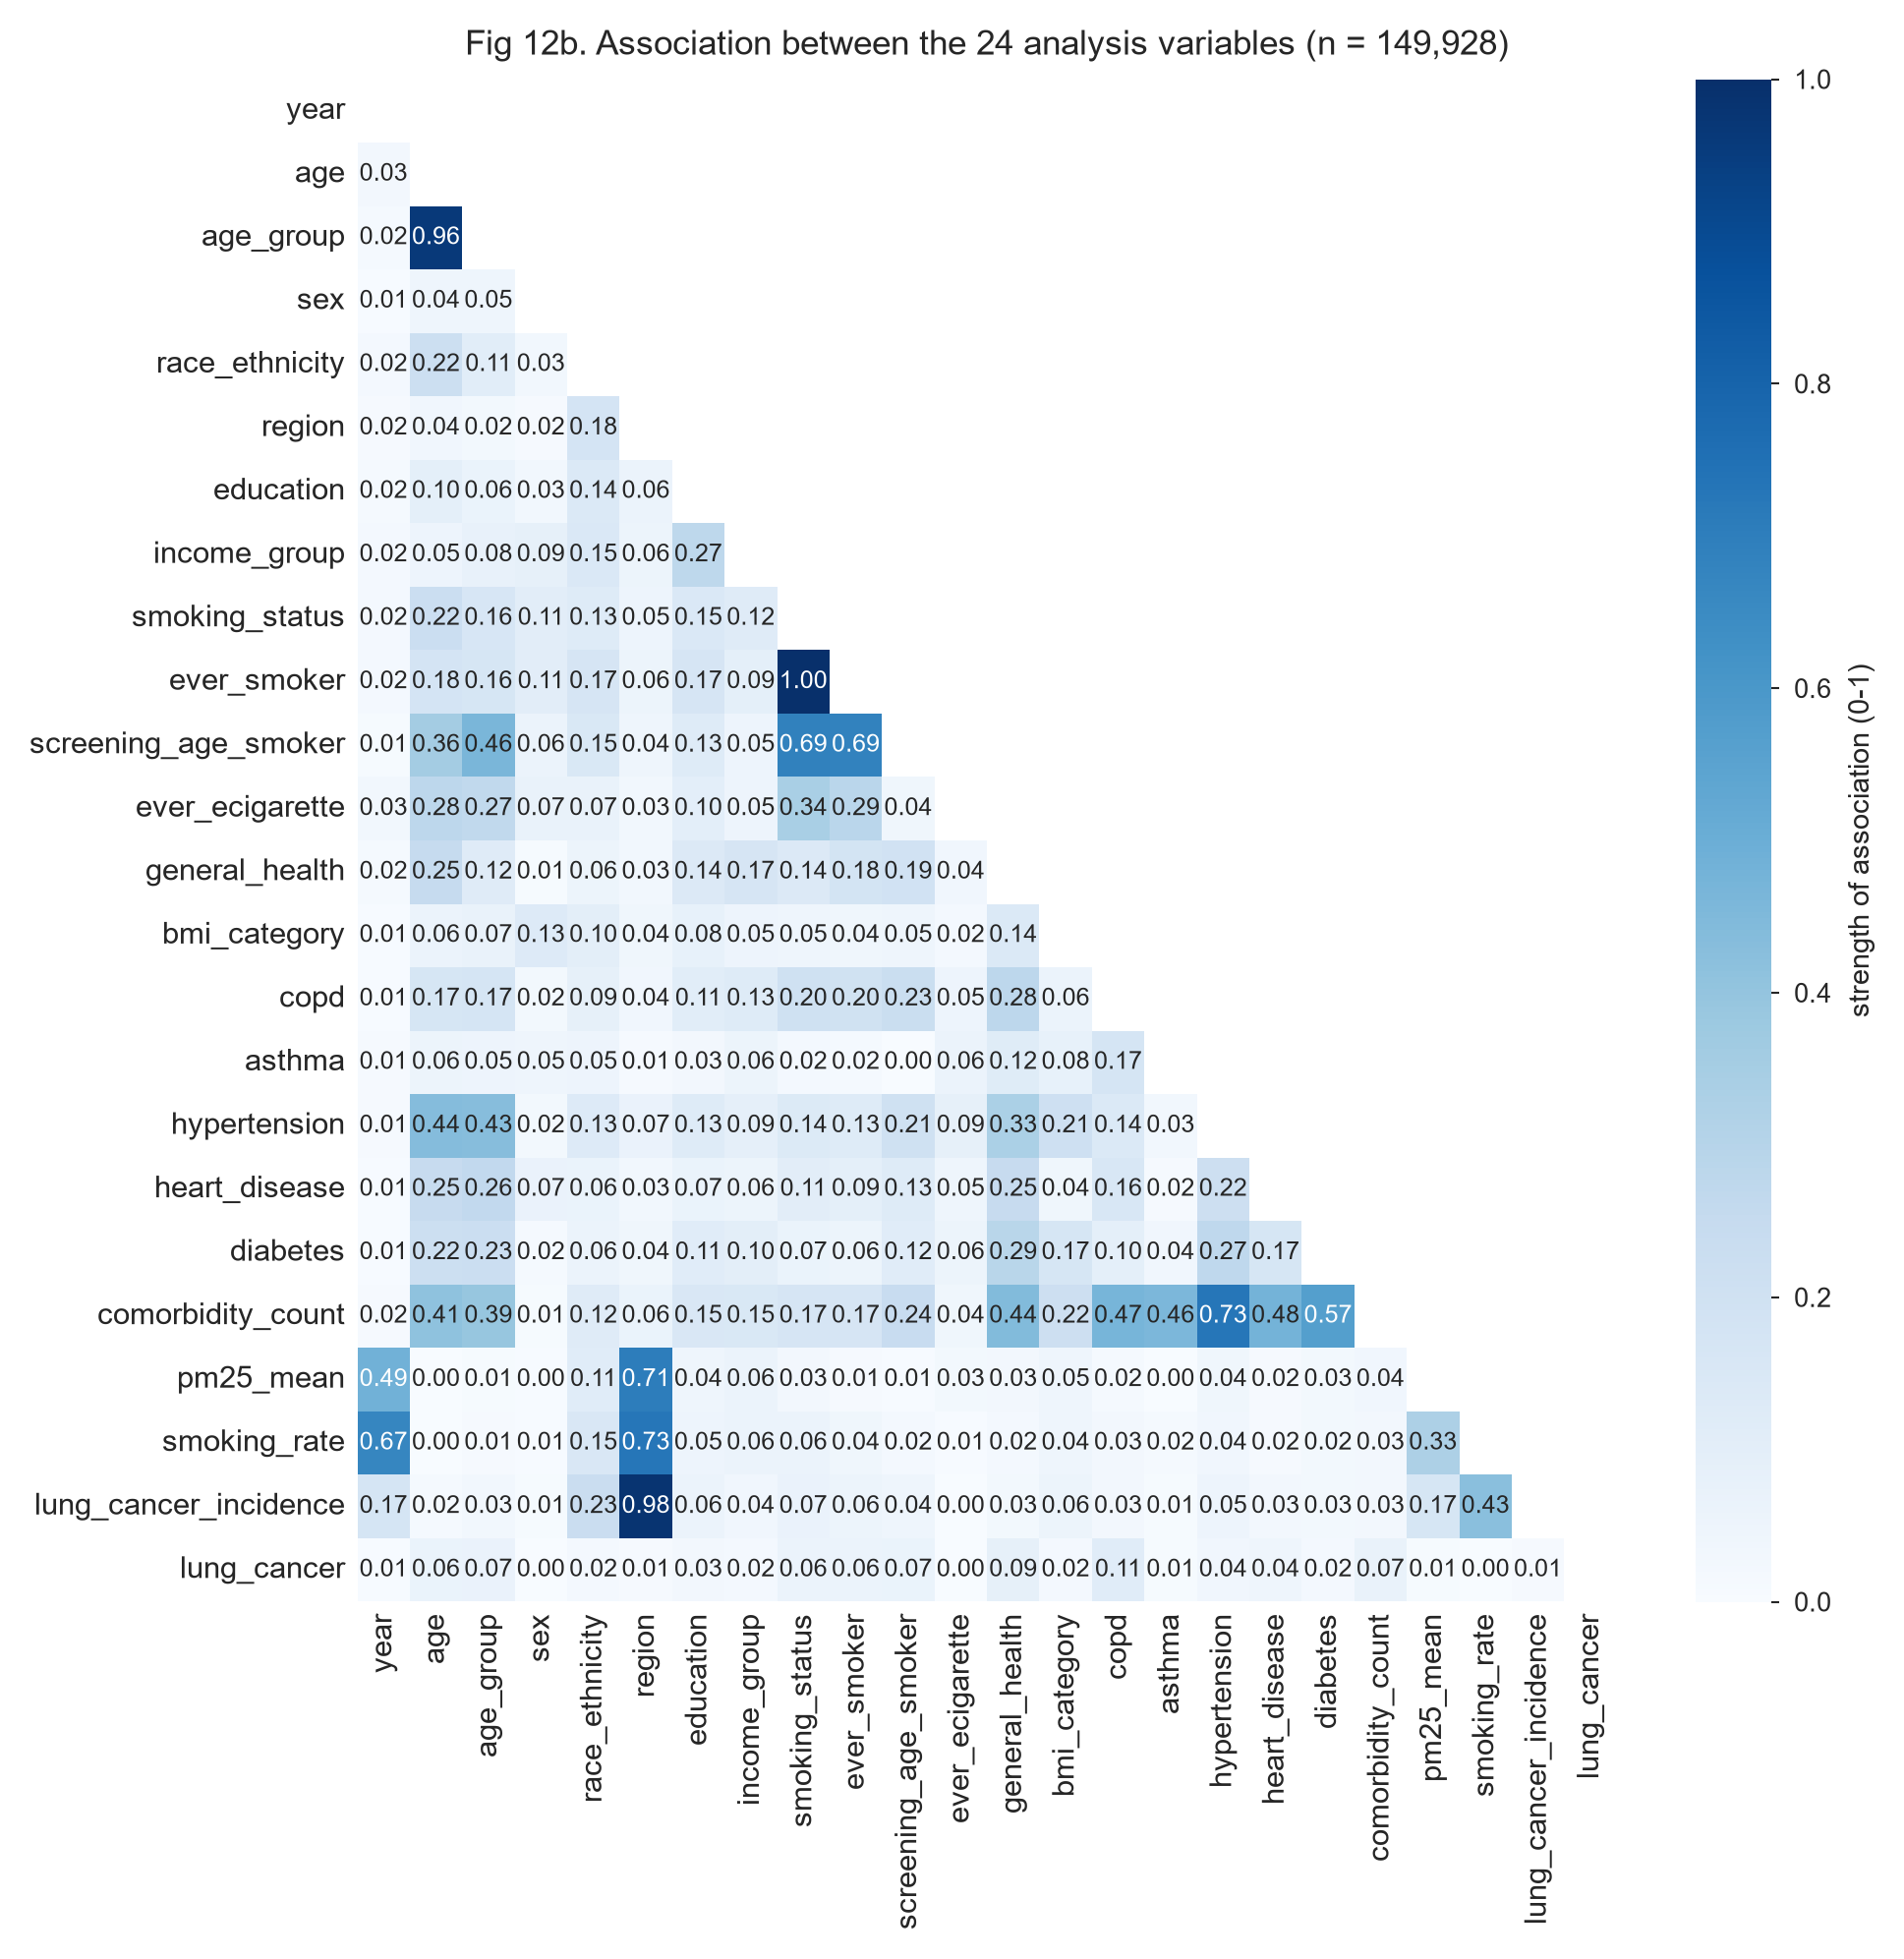
\includegraphics[width=\textwidth]{fig12b_association_matrix}
\figsuffix{b}
\caption{Association between all 24 analysis variables of the clean dataset and the target (all \nAdults adults, \nCases cases; each pair uses the adults with both values known, $n$ = 142,511--149,928; unweighted). Cram\'er's $V$ for two categorical variables, the correlation ratio $\eta$ for a categorical and a numeric variable, $|\text{Spearman}|$ for two numeric variables; all three run from 0 to 1. \texttt{person\_id} and \texttt{survey\_weight} are excluded, and \texttt{CANEV\_A} is not in the clean dataset.}\label{fig:assoc}
\end{figure}

\begin{figure}[p]
\centering
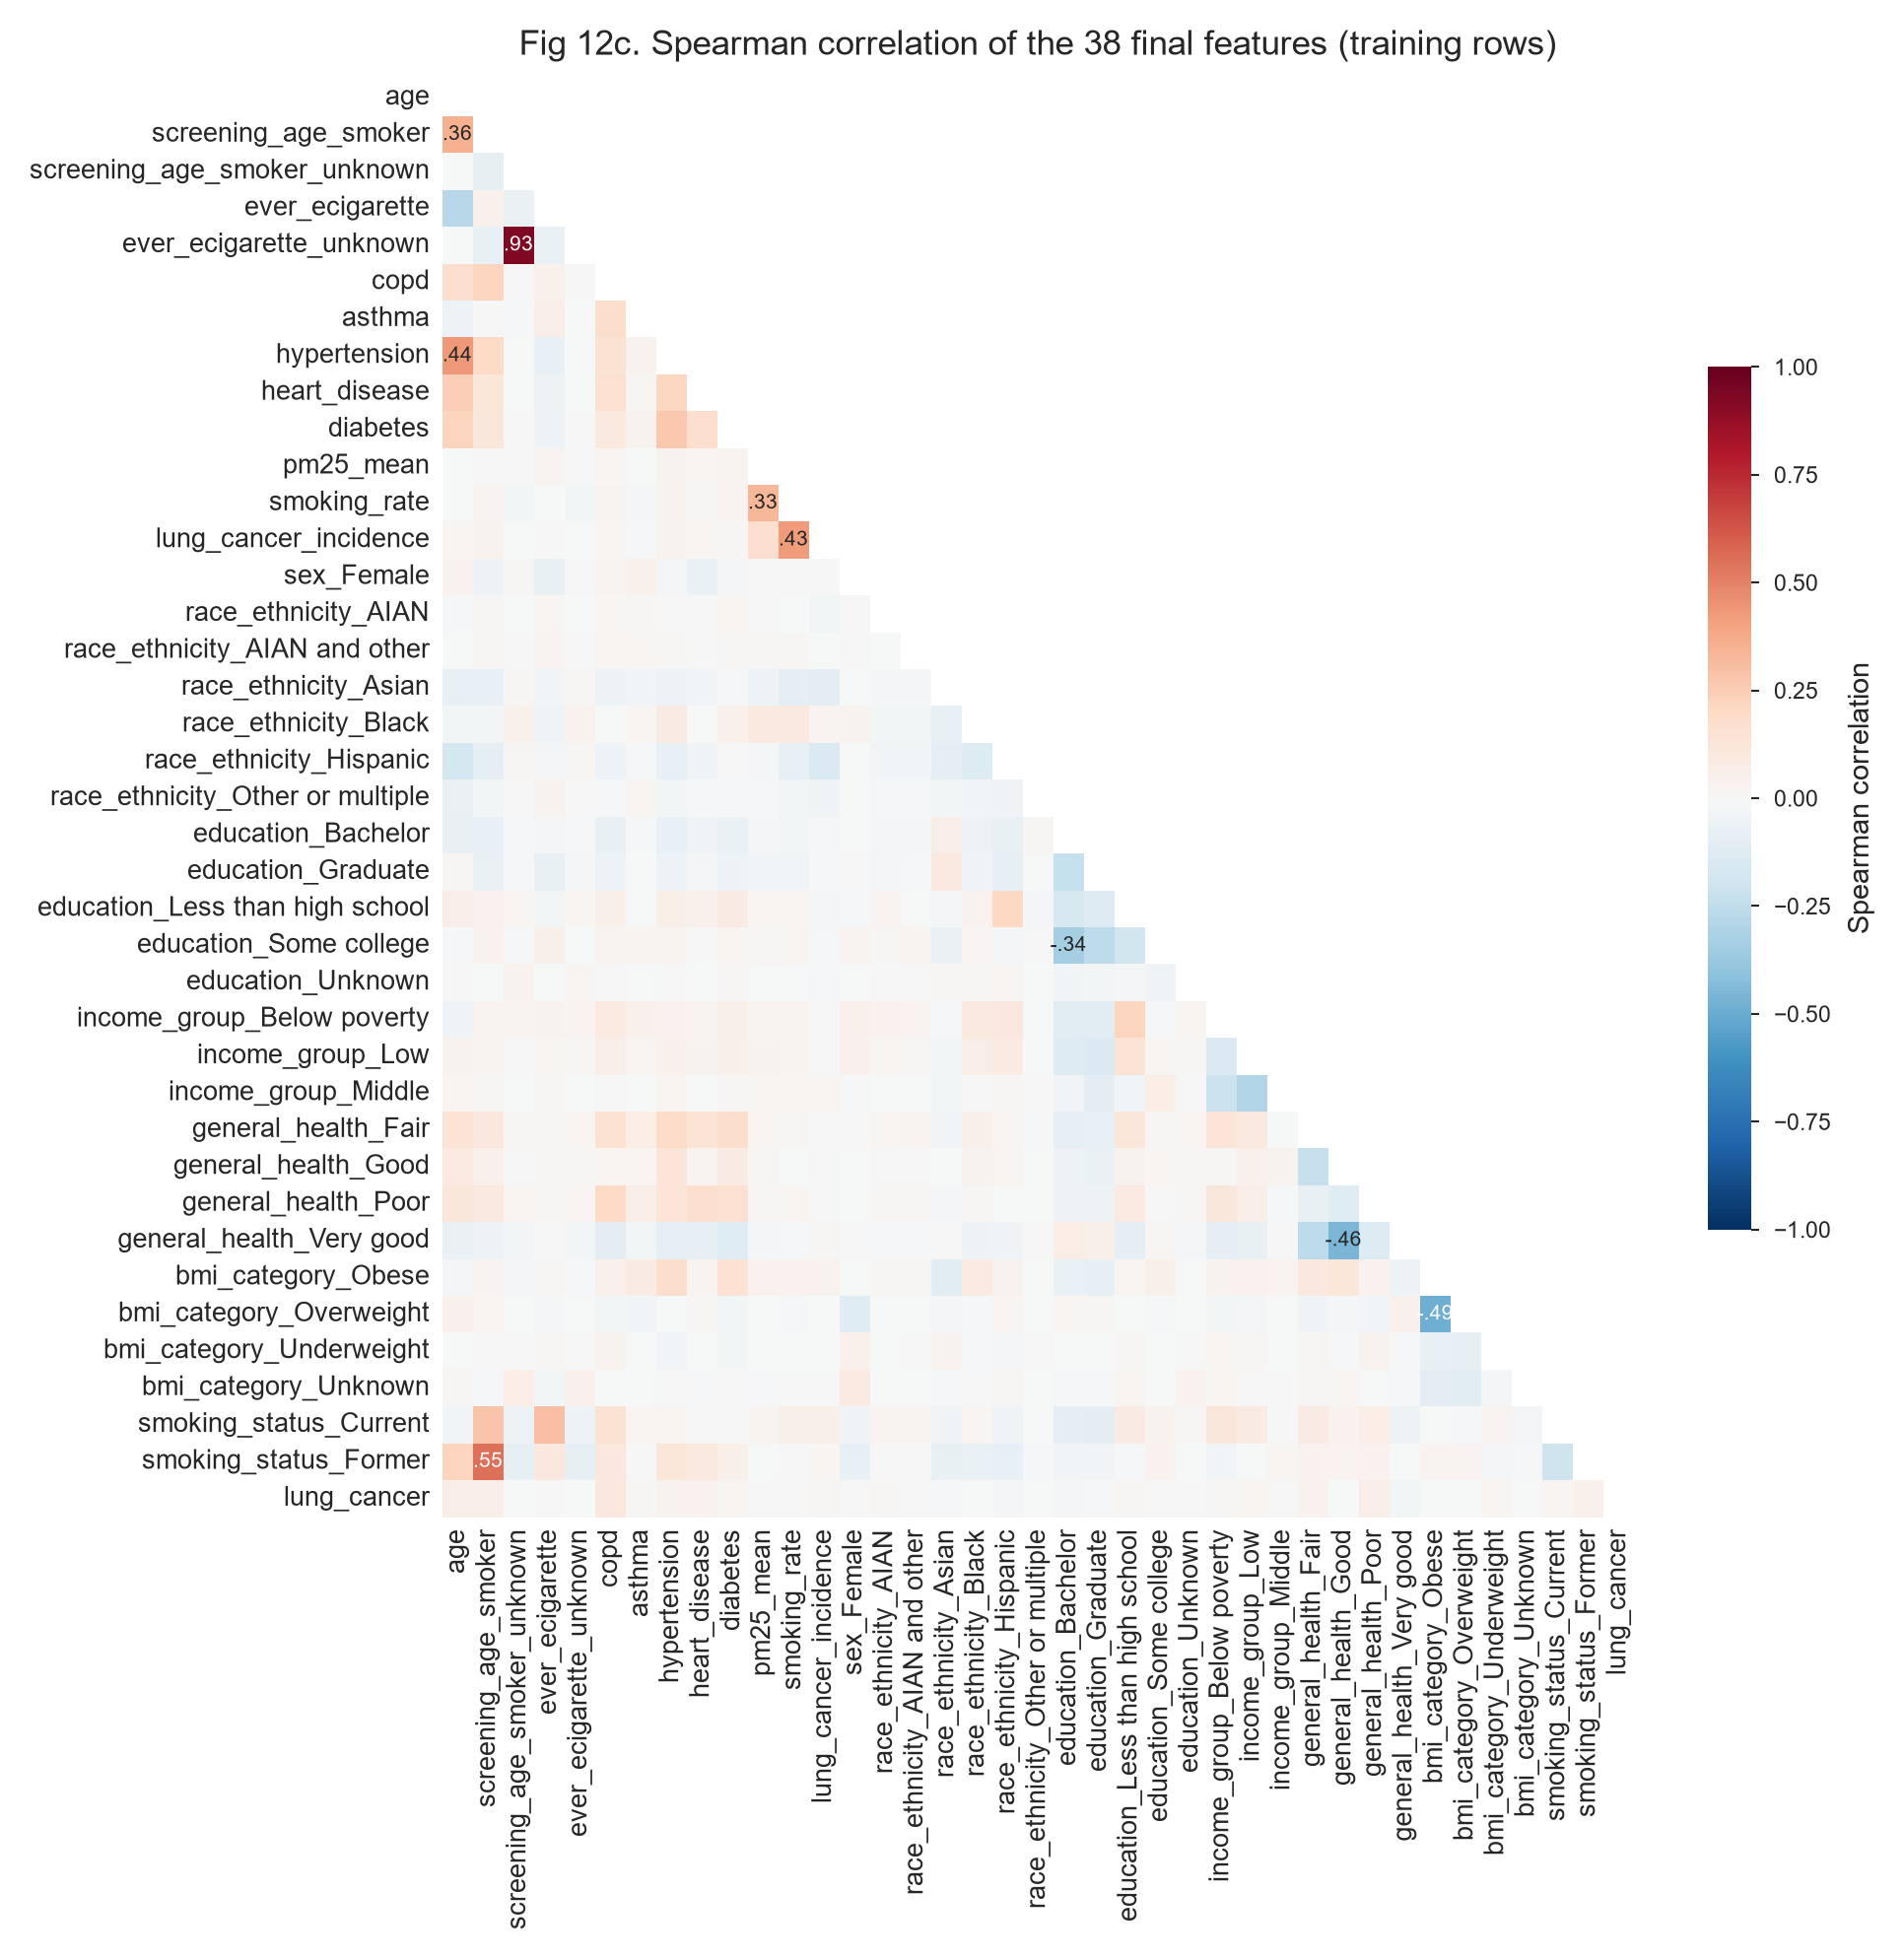
\includegraphics[width=\textwidth]{fig12c_feature_correlation}
\figsuffix{c}
\caption{Spearman correlation of the \nFeatures final model features and the target, on the training rows only ($n$ = \nTrain adults, \nTrainCases cases; unweighted; lower triangle; values printed where $|r| \geq 0.3$).}\label{fig:featcorr}
\end{figure}

Fig.~\ref{fig:corr} only holds the numeric and 0/1 columns, so it cannot show how the categorical variables relate to each other or to the target. Fig.~\ref{fig:assoc} therefore covers \emph{all} 24 analysis variables, with the measure that suits each pair of types, and Fig.~\ref{fig:featcorr} covers \emph{all} \nFeatures features handed to the modelling phase. Every pair above 0.5 in either matrix is listed in Table~\ref{tab:high-pairs} with the reason it is high (\file{results/tables/high_correlation_pairs.csv}).

\begin{table}[htbp]
\centering\footnotesize
\caption{Every pair of variables (Fig.~\ref{fig:assoc}) or features (Fig.~\ref{fig:featcorr}) with an association above 0.5.}\label{tab:high-pairs}
\begin{tabularx}{\textwidth}{l >{\raggedright\arraybackslash}p{4.2cm} l r l >{\raggedright\arraybackslash}X}
\toprule
Matrix & Pair & Measure & Value & Type & Why it is high \\
\midrule
Fig.~12b & year -- smoking\_\allowbreak{}rate & $\eta$ & 0.67 & built-from & smoking\_rate is joined on region + year, and BRFSS smoking fell every year 2019--2023 \\
Fig.~12b & age -- age\_\allowbreak{}group & $\eta$ & 0.96 & built-from & age\_group is age cut into bands \\
Fig.~12b & region -- pm25\_\allowbreak{}mean & $\eta$ & 0.71 & built-from & pm25\_mean is joined on region + year (20 values) \\
Fig.~12b & region -- smoking\_\allowbreak{}rate & $\eta$ & 0.73 & built-from & smoking\_rate is joined on region + year (20 values) \\
Fig.~12b & region -- lung\_\allowbreak{}cancer\_\allowbreak{}incidence & $\eta$ & 0.98 & built-from & lung\_cancer\_incidence is joined on region + year; the West is far lower than the other regions \\
Fig.~12b & smoking\_\allowbreak{}status -- ever\_\allowbreak{}smoker & Cram\'er's $V$ & 1.00 & built-from & ever\_smoker = Current or Former smoking\_status \\
Fig.~12b & smoking\_\allowbreak{}status -- screening\_\allowbreak{}age\_\allowbreak{}smoker & Cram\'er's $V$ & 0.69 & built-from & screening\_age\_smoker = aged 50--80 AND ever smoked \\
Fig.~12b & ever\_\allowbreak{}smoker -- screening\_\allowbreak{}age\_\allowbreak{}smoker & Cram\'er's $V$ & 0.69 & built-from & screening\_age\_smoker = aged 50--80 AND ever smoked \\
Fig.~12b & hypertension -- comorbidity\_\allowbreak{}count & $\eta$ & 0.73 & built-from & comorbidity\_count is the sum of the 5 condition flags, hypertension the most common (36.5\%) \\
Fig.~12b & diabetes -- comorbidity\_\allowbreak{}count & $\eta$ & 0.57 & built-from & comorbidity\_count is the sum of the 5 condition flags \\
Fig.~12c & screening\_\allowbreak{}age\_\allowbreak{}smoker\_\allowbreak{}unknown -- ever\_\allowbreak{}ecigarette\_\allowbreak{}unknown & Spearman & 0.93 & same-concept & both flag the same $\sim$2.8\% of adults who skipped the smoking / tobacco questions \\
Fig.~12c & screening\_\allowbreak{}age\_\allowbreak{}smoker -- smoking\_\allowbreak{}status\_\allowbreak{}Former & Spearman & 0.55 & built-from & screening\_age\_smoker is built from smoking status, and most former smokers are aged 50--80 \\
\bottomrule
\end{tabularx}

\end{table}

\begin{itemize}
  \item \textbf{Redundancy -- what is high, and what we did about it.} All twelve pairs above 0.5 are either \emph{built-from} (one column is computed from the other, or both are joined on region + year; 11 pairs) or \emph{same-concept} (two flags for the same missing block; 1 pair). \textbf{No two separately measured personal variables are associated above 0.5.} The built-from overlaps are handled in feature selection: \file{ever_smoker} and the age bands are dropped by rule 1, and \file{comorbidity_count} and the region dummies by the new rule 4 (\S\ref{sec:selection}). The two high pairs left among the final features are kept on purpose: the two ``unknown'' flags, which together identify adults with an unknown smoking status (\S\ref{sec:final}), and \file{screening_age_smoker} with former smoking, because the screening rule needs smoking status and age together. Both have a variance inflation factor below 10 (Table~\ref{tab:vif}). Pairwise matrices also have a blind spot: a column can be an exact combination of \emph{several} others (the comorbidity count is the sum of five flags; every complete one-hot group sums to 1) without any single pair exceeding 0.5. Hypertension--comorbidity count was the only visible trace of such a dependency in Fig.~\ref{fig:corr} (Spearman 0.79). This is why feature selection now also checks the VIF (\S\ref{sec:selection}).
  \item \textbf{Why every correlation with the target is small.} Nothing correlates strongly with the target (Fig.~\ref{fig:corr}: highest COPD 0.11, age 0.07; Fig.~\ref{fig:assoc}: COPD 0.11, general health 0.09). This is a property of a rare outcome, not a sign that the factors are weak. For two 0/1 variables, Spearman, Pearson and $\varphi$ coincide, and $\varphi$ can only reach 1 when both have the same prevalence. A feature with prevalence $q$ can reach at most $\varphi_{\max} = \sqrt{p(1-q) / \bigl(q(1-p)\bigr)}$ with a target of prevalence $p = \sampleRate\%$. COPD (5.6\% of adults) can therefore reach at most 0.26, and its observed 0.11 is 43\% of that maximum, with an odds ratio of \orCOPD (Table~\ref{tab:target-bound}). Ever-smoking reaches 71\% of its maximum of 0.08. Correlations with this target must therefore be read together with the odds ratios and rates of \S\ref{sec:rq1}--\ref{sec:sociodemo}, never on their own. Because no single feature is strongly associated with the target, a model will need to combine them.
\end{itemize}

\begin{table}[htbp]
\centering\small
\caption{Observed and largest possible correlation ($\varphi$) between each 0/1 factor and the target, with the odds ratio (all adults with the factor known; unweighted; source: \texttt{target\_correlation\_bound.csv}).}\label{tab:target-bound}
\begin{tabular}{lrrrrrr}
\toprule
Factor & Adults (cases) & Prevalence & \makecell[b]{$\varphi$\\{}observed} & $\varphi_{\max}$ & \makecell[b]{Share\\{}of max} & \makecell[b]{Odds\\{}ratio} \\
\midrule
COPD & 149,826 (618) & 5.6\% & 0.114 & 0.263 & 43\% & 15.1 \\
Heart disease & 149,597 (614) & 6.1\% & 0.045 & 0.253 & 18\% & 4.6 \\
Hypertension & 149,766 (619) & 36.6\% & 0.038 & 0.085 & 45\% & 3.3 \\
Diabetes & 149,860 (619) & 10.7\% & 0.022 & 0.186 & 12\% & 2.3 \\
Asthma & 149,864 (618) & 13.9\% & 0.009 & 0.160 & 6\% & 1.4 \\
Ever smoked & 145,975 (601) & 37.7\% & 0.059 & 0.083 & 71\% & 7.7 \\
Screening-age smoker & 145,664 (600) & 22.2\% & 0.066 & 0.120 & 55\% & 6.5 \\
E-cigarette (ever) & 146,076 (602) & 16.1\% & 0.002 & 0.147 & 2\% & 1.1 \\
\bottomrule
\end{tabular}

\end{table}

\subsection{RQ3 -- Regional factors}\label{sec:regional}

\begin{figure}[htbp]
\centering
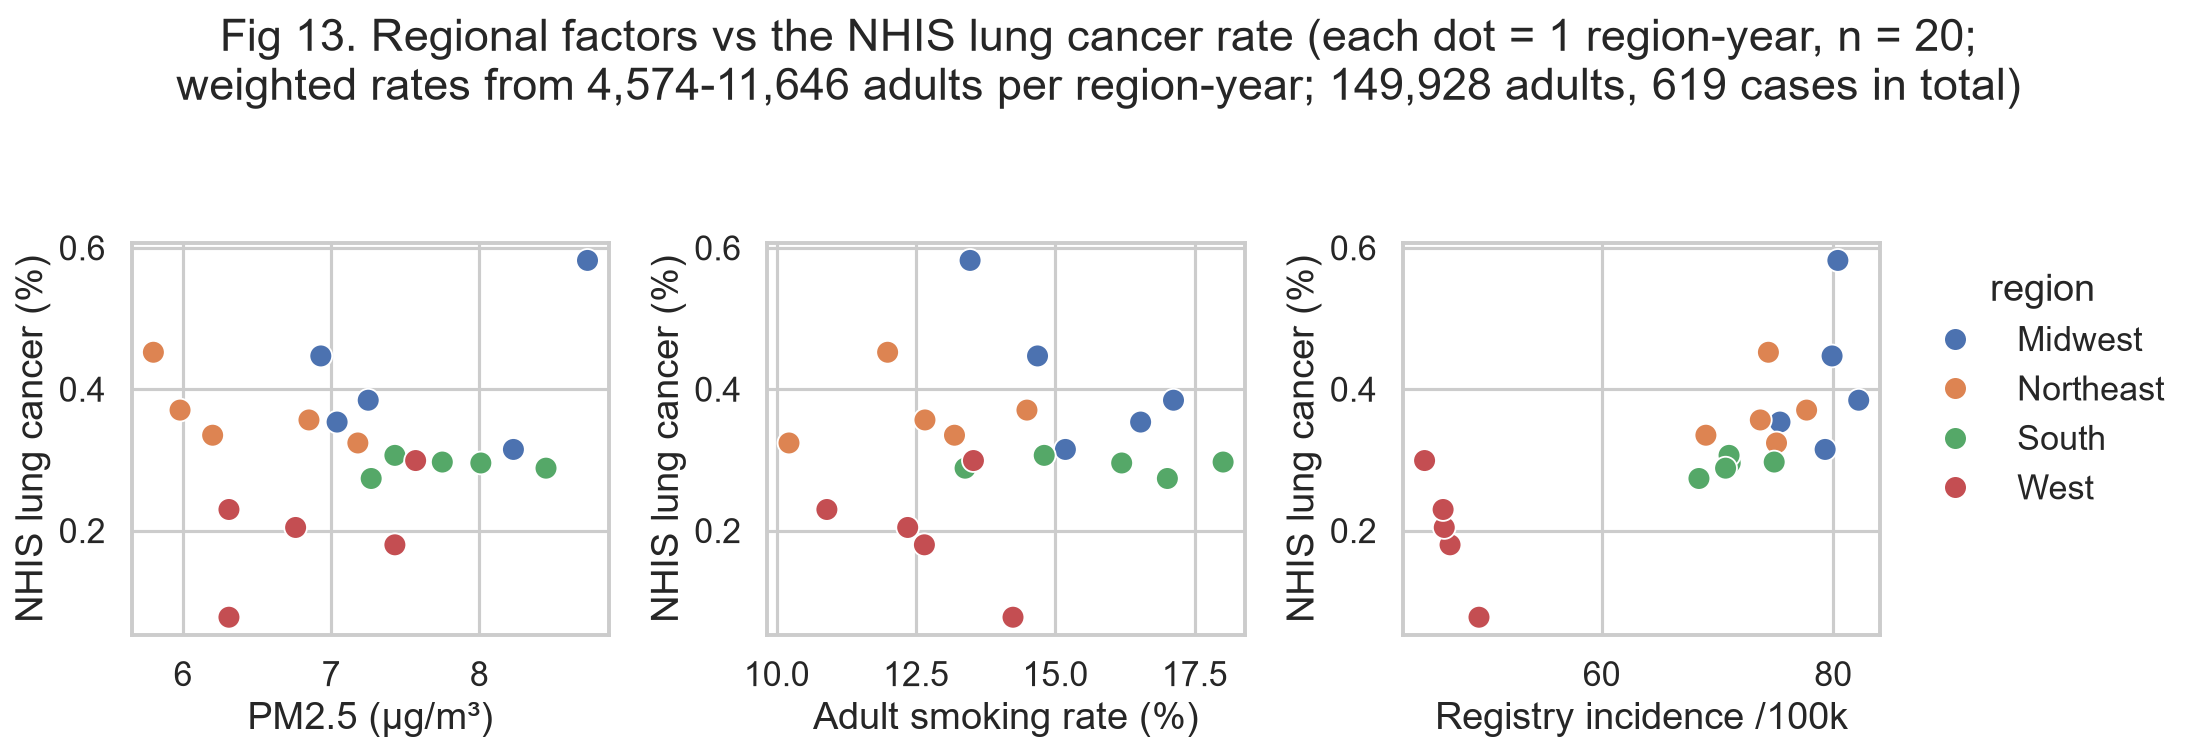
\includegraphics[width=\textwidth]{fig13_regional_factors}
\caption{Regional PM2.5, adult smoking rate and registry incidence against the weighted NHIS lung-cancer rate. Each dot is one region-year ($n$ = 20: 4 regions $\times$ 5 years); each region-year rate is the survey-weighted rate of its adults (\regionYearMin to \regionYearMax adults per region-year; \nAdults adults and \nCases cases in total).}\label{fig:regional}
\end{figure}

\begin{itemize}
  \item \textbf{The cross-source check.} Over the 20 region-years, the survey-based rate follows the official registry incidence (Fig.~\ref{fig:regional}; Spearman $\rho = \rhoRegistry$, $p$ = \pRegistry, Holm $p$ = \holmRegistry). Pooled over five years, the weighted rate is highest in the Midwest (0.42\%) and Northeast (0.37\%) and lowest in the West (0.20\%), the region with by far the lowest registry incidence (46.7 per 100,000 against 71--79 elsewhere).
  \item \textbf{Why we read it cautiously.} The 20 points are four regions measured five times, so they are not independent. Table~\ref{tab:regional} splits the correlation in two: the four regional means rank identically on both measures ($\rho = 1.0$, but $n = 4$), while the year-to-year changes within a region do not move together ($\rho = 0.03$, $p = 0.89$). The agreement is therefore mainly ``the West is low on both measures''. It is consistent with our self-reported target behaving like the official statistic, but it is not a formal validation, and its $p$-value is optimistic. The two measures also differ in kind -- lifetime history vs new cases per year. For PM2.5 and the regional smoking rate, the between-region correlation in Table~\ref{tab:regional} is exactly 0.00. This is a real value, not a computation error: both measures rank the four regions differently from the NHIS rate, the squared rank differences add up to exactly 10, and $\rho = 1 - 6 \times 10 / (4 \times 15) = 0$. With only four points, $\rho$ can take just a few values ($0, \pm 0.2, \pm 0.4, \ldots, \pm 1$), so this zero says nothing either way.
  \item \textbf{Air pollution and regional smoking rates show no association} (PM2.5: $\rho = -0.12$, $p = 0.63$; smoking rate: $\rho = 0.09$, $p = 0.71$), neither between nor within regions. With so few independent data points these tests are underpowered, so ``no evidence'' does not mean ``no effect''.
  \item \textbf{Why a null result is expected here.} The registry rate is crude, not age-adjusted (the West has a younger population); state values are averaged without population weights; and 2019--2023 pollution cannot explain cancers diagnosed many years earlier. Regional averages also say nothing about any individual (the ecological fallacy).
  \item \textbf{Do they add information beyond personal factors?} Mutual information on training rows (\S\ref{sec:mi}) puts all three regional columns far below the personal factors: about 0.5--0.6\% of the target's information, against 10.2\% for age. Their scores are above a shuffled-target noise level, but tiny. The three scores also measure the same thing. As discrete features, the regional values only say \emph{which region-year} a person lives in: \file{smoking_rate} and \file{lung_cancer_incidence} take a different value in each of the 20 region-years, so their mutual information is exactly that of the region-year label (0.00017 nats each), and PM2.5, where two pairs of region-years share a value, is slightly lower (0.00014). So the data cannot tell whether pollution, regional smoking or registry incidence matters; at this resolution the three columns together add one small region-year signal.
\end{itemize}

\begin{table}[htbp]
\centering\small
\caption{Spearman correlation of each regional measure with the weighted NHIS lung-cancer rate: over all 20 region-years, between the 4 regional means, and within regions (year-to-year deviations from each region's mean). Between-region values use $n = 4$, so $\rho$ can only take a few values; the 0.00 for PM2.5 and smoking rate is exact (see text). Source: \texttt{regional\_within\_between.csv}.}\label{tab:regional}
\begin{tabular}{lrrr}
\toprule
Regional measure & \makecell[b]{All 20\\{}region-years} & \makecell[b]{Between\\{}4 regions} & \makecell[b]{Within regions\\{}($n$ = 20)} \\
\midrule
PM2.5 & $-$0.12 ($p$ = 0.63) & 0.00 & 0.03 ($p$ = 0.89) \\
Regional smoking rate & 0.09 ($p$ = 0.71) & 0.00 & $-$0.35 ($p$ = 0.13) \\
Registry incidence & 0.79 ($p$ = $3.5\times10^{-5}$) & 1.00 & 0.03 ($p$ = 0.89) \\
\bottomrule
\end{tabular}

\end{table}

\subsection{All tests, with multiple-testing correction}\label{sec:alltests}

Running eighteen tests raises the chance of a false positive, so we corrected all of them together with the Holm method~\cite{holm} (Table~\ref{tab:all-tests}), which keeps the family-wise error rate at 5\% and is uniformly more powerful than Bonferroni.

\begin{table}[htbp]
\centering\small
\caption{All \nTests hypothesis tests with raw and Holm-adjusted $p$-values, labelled with the research question each one answers (\texttt{results/tables/all\_tests\_holm.csv}). $^{a}$The 20 region-years are not independent (4 regions $\times$ 5 years), so this $p$-value is optimistic; see \S\ref{sec:regional} and Table~\ref{tab:regional}.}\label{tab:all-tests}
\begin{tabularx}{\textwidth}{l >{\raggedright\arraybackslash}X r r l}
\toprule
RQ & Test & $p$ & Holm $p$ & Significant \\
\midrule
RQ1 & Smoking status ($\chi^2$) & $2.2\times10^{-115}$ & $3.1\times10^{-114}$ & yes \\
RQ2a & Age (Mann--Whitney $U$) & $3.1\times10^{-141}$ & $4.6\times10^{-140}$ & yes \\
RQ2b & COPD ($\chi^2$) & $<10^{-300}$ & $<10^{-300}$ & yes \\
RQ2b & COPD adjusted for smoking (CMH) & $1.5\times10^{-208}$ & $2.4\times10^{-207}$ & yes \\
RQ2b & Heart disease ($\chi^2$) & $5.6\times10^{-66}$ & $7.3\times10^{-65}$ & yes \\
RQ2b & Hypertension ($\chi^2$) & $1.3\times10^{-49}$ & $1.5\times10^{-48}$ & yes \\
RQ2b & Diabetes ($\chi^2$) & $6.7\times10^{-17}$ & $6.7\times10^{-16}$ & yes \\
RQ2b & Asthma ($\chi^2$) & $5.7\times10^{-4}$ & $2.9\times10^{-3}$ & yes \\
RQ2b & E-cigarette, ever ($\chi^2$) & 0.39 & 1.00 & no \\
RQ2c & Sex ($\chi^2$) & 0.16 & 0.62 & no \\
RQ2c & Race / ethnicity ($\chi^2$) & $1.6\times10^{-14}$ & $1.1\times10^{-13}$ & yes \\
RQ2c & Education ($\chi^2$) & $7.1\times10^{-24}$ & $7.8\times10^{-23}$ & yes \\
RQ2c & Income vs poverty line ($\chi^2$) & $8.3\times10^{-17}$ & $7.5\times10^{-16}$ & yes \\
RQ2c & BMI category ($\chi^2$) & $6.5\times10^{-15}$ & $5.2\times10^{-14}$ & yes \\
RQ2c & Self-rated general health ($\chi^2$) & $1.1\times10^{-248}$ & $1.8\times10^{-247}$ & yes \\
RQ3 & PM2.5 vs regional rate (Spearman, $n$ = 20) & 0.63 & 1.00 & no \\
RQ3 & Smoking rate vs regional rate (Spearman, $n$ = 20) & 0.71 & 1.00 & no \\
RQ3 & Registry incidence vs regional rate (Spearman, $n$ = 20)$^{a}$ & $3.5\times10^{-5}$ & $2.1\times10^{-4}$ & yes \\
\bottomrule
\end{tabularx}

\end{table}

\nSignificant of \nTests tests remain significant after correction (RQ1: 1 test, RQ2a: 1, RQ2b: 7, RQ2c: 6, RQ3: 3). The four that do not -- e-cigarette use, sex, PM2.5 and the regional smoking rate -- are discussed above. The COPD $\chi^2$ $p$-value is reported as ``$<10^{-300}$'' because it is below the smallest number the computer can represent ($\chi^2 \approx 1{,}950$ with 1 degree of freedom). For the CMH test we compute the $p$-value from the $\chi^2$ survival function, because the library's default returns 0 for such large statistics.

\textbf{Survey-design sensitivity.} Our tests treat respondents as independent draws, but NHIS is a stratified, clustered sample. To check how much this matters, \file{supplementary_analysis.py} reads the NHIS design variables (\file{PSTRAT}, \file{PPSU}) from the raw files and re-estimates the three key associations with survey-weighted logistic regression and confidence intervals clustered on the 3,160 sampling units (Table~\ref{tab:design}). The weighted odds ratios are somewhat larger than the unweighted ones, the interval widths change by a factor of 0.9 to 1.2, and every interval stays far from 1. The conclusions therefore do not depend on ignoring the design; a fully design-based analysis of every test remains a next step. The rates in our figures are survey-weighted.

\begin{table}[htbp]
\centering\small
\caption{Survey-design sensitivity: odds ratios from unweighted logistic regression (exact; the $2 \times 2$ tables elsewhere add 0.5 to each cell, e.g.\ 7.66 instead of 7.69 for smoking) and from survey-weighted logistic regression with confidence intervals clustered on the NHIS sampling units (year $\times$ stratum $\times$ PSU). Source: \texttt{design\_based\_odds\_ratios.csv}.}\label{tab:design}
\begin{tabular}{lrrr}
\toprule
Exposure & Adults & \makecell[b]{Unweighted OR\\{}[95\% CI]} & \makecell[b]{Weighted, clustered\\{}OR [95\% CI]} \\
\midrule
Ever smoked (vs never) & 145,975 & 7.69 [6.24, 9.48] & 9.14 [7.17, 11.65] \\
COPD (vs none) & 149,826 & 15.10 [12.87, 17.71] & 18.64 [15.43, 22.53] \\
Age, per 10 years & 149,575 & 2.03 [1.91, 2.16] & 2.15 [2.03, 2.27] \\
\bottomrule
\end{tabular}

\end{table}

\subsection{What the statistics do not show}\label{sec:notshow}

\begin{itemize}
  \item \textbf{No causes.} Every result here is an association in cross-sectional survey data. That smoking causes lung cancer is established elsewhere~\cite{uspstf,tammemagi}; our data only show a pattern consistent with it.
  \item \textbf{No individual risk.} A \orSmoking\unskip$\times$ odds ratio describes groups. It does not say how likely any one person is to develop lung cancer, and the regional results say nothing about individuals at all.
  \item \textbf{No dose--response.} Without pack-years we cannot test whether more smoking means more risk, which is the core of real screening rules.
  \item \textbf{``Not significant'' is not ``no effect''.} For e-cigarettes we ran a power check: with 23,470 ever-users, 122,606 never-users and a \sampleRate\% base rate, the test had 80\% power ($\alpha = 0.05$) to detect an odds ratio of about 1.34 or larger. So we can rule out a large effect in these data, but not a small one, and certainly not a long-term one that has not had time to appear.
  \item \textbf{Limited adjustment.} Smoking was adjusted for age, and COPD for smoking and age, by stratification. The other odds ratios are crude, so part of each one is age; a multivariable model (\S\ref{sec:next}) is needed to separate them all at once.
\end{itemize}
